% !TeX document-id = {54d2d254-7585-48d2-9f78-dac02ef9b770}
% !TeX spellcheck = en-US
% !TeX encoding = utf8
% !TeX program = lualatex
% !BIB program = biber
% -*- coding:utf-8 mod:LaTeX -*-


% vv  scroll down to line 200 for content  vv

\PassOptionsToPackage{language=english}{uni-stuttgart-cs-cover}

\let\ifdeutsch\iffalse
\let\ifenglisch\iftrue
\input{pre-documentclass}
\documentclass[
  % fontsize=11pt is the standard
  a4paper,  % Standard format - only KOMAScript uses paper=a4 - https://tex.stackexchange.com/a/61044/9075
  twoside,  % we are optimizing for both screen and two-side printing. So the page numbers will jump, but the content is configured to stay in the middle (by using the geometry package)
  bibliography=totoc,
  %               idxtotoc,   %Index ins Inhaltsverzeichnis
  %               liststotoc, %List of X ins Inhaltsverzeichnis, mit liststotocnumbered werden die Abbildungsverzeichnisse nummeriert
  headsepline,
  cleardoublepage=empty,
  parskip=half,
  %               draft    % um zu sehen, wo noch nachgebessert werden muss - wichtig, da Bindungskorrektur mit drin
  draft=false
]{scrbook}
% !TeX encoding = utf8
% -*- coding:utf-8 mod:LaTeX -*-

% EN: This file includes basic packages and sets options. The order of package
%     loading is important

% DE: In dieser Datei werden zuerst die benoetigten Pakete eingebunden und
%     danach diverse Optionen gesetzt. Achtung Reihenfolge ist entscheidend!


% EN: Styleguide:
% - English comments are prefixed with "EN", German comments are prefixed with "DE"
% - Prefixed headings define the language for the subsequent paragraphs
% - It is tried to organize packages in blocks. Bocks are separated by two empty lines.

% DE: Styleguide:
%
% Ein sehr kleiner Styleguide. Packages werden in Blöcken organisiert.
% Zwischen zwei Blöcken sind 2 Leerzeilen!


% EN: Enable copy and paste of text from the PDF
%     Only required for pdflatex. It "just works" in the case of lualatex.
%     mmap enables mathematical symbols, but does not work with the newtx font set
%     See: https://tex.stackexchange.com/a/64457/9075
%     Other solutions outlined at http://goemonx.blogspot.de/2012/01/pdflatex-ligaturen-und-copynpaste.html and http://tex.stackexchange.com/questions/4397/make-ligatures-in-linux-libertine-copyable-and-searchable
%     Trouble shooting outlined at https://tex.stackexchange.com/a/100618/9075

\ifluatex
\else
  \usepackage{cmap}
\fi


% EN: File encoding
% DE: Codierung
%     Wir sind im 21 Jahrhundert, utf-8 löst so viele Probleme.
%
% Mit UTF-8 funktionieren folgende Pakete nicht mehr. Bitte beachten!
%   * fancyvrb mit §
%   * easylist -> http://www.ctan.org/tex-archive/macros/latex/contrib/easylist/
\ifluatex
  % EN: See https://tex.stackexchange.com/a/158517/9075
  %     Not required, because of usage of fontspec package
  %\usepackage[utf8]{luainputenc}
\else
  \usepackage[utf8]{inputenc}
\fi


% DE: Parallelbetrieb tex4ht und pdflatex

\makeatletter
\@ifpackageloaded{tex4ht}{
  \def\iftex4ht{\iftrue}
}{
  \def\iftex4ht{\iffalse}
}
\makeatother


% EN: Mathematics
% DE: Mathematik
%
% DE: Viele Mathematik-Sachen. Siehe https://texdoc.net/pkg/amsmath
%
% EN: Options must be passed this way, otherwise it does not work with glossaries
% DE: fleqn (=Gleichungen linksbündig platzieren) funktioniert nicht direkt. Es muss noch ein Patch gemacht werden:
\PassOptionsToPackage{fleqn,leqno}{amsmath}
%
% DE: amsmath Muss nicht mehr geladen werden, da es von newtxmath automatisch geladen wird
% \usepackage{amsmath}


%% EN: Fonts
%% DE: Schriften
%%
%% !!! If you change the font, be sure that words such as "workflow" can
%% !!! still be copied from the PDF. If this is not the case, you have
%% !!! to use glyphtounicode. See comment at cmap package


% EN: Times Roman for all text
\ifluatex
  % source: Second proposed fix from the following answer: https://tex.stackexchange.com/a/394137
  \usepackage[no-math]{fontspec}
  \setmainfont{TeXGyreTermes-Regular}[
       BoldFont       = TeXGyreTermes-Bold ,
       ItalicFont     = TeXGyreTermes-Italic ,
       BoldItalicFont = TeXGyreTermes-BoldItalic,
       NFSSFamily     = ntxtlf]
  \setsansfont{TeX Gyre Heros Regular}[
       Scale=.9,
       BoldFont       = TeX Gyre Heros Bold,
       ItalicFont     = TeX Gyre Heros Italic,
       BoldItalicFont = TeX Gyre Heros BoldItalic]
  \setmonofont[StylisticSet={1,3},Scale=.9]{inconsolata}
  \RequirePackage{newtxmath}
\else
  \RequirePackage{newtxtext}
  \RequirePackage{newtxmath}
  % EN: looks good with times, but no equivalent for lualatex found,
  %     therefore replaced with inconsolata
  %\RequirePackage[zerostyle=b,scaled=.9]{newtxtt}
  \RequirePackage[varl,scaled=.9]{inconsolata}
\fi

% EN: Fallback font - if the subsequent font packages do not define a font (e.g., monospaced)
%     This is the modern package for "Computer Modern".
%     In case this gets activated, one has to switch from cmap package to glyphtounicode (in the case of pdflatex)
% DE: Fallback-Schriftart
%\usepackage[%
%    rm={oldstyle=false,proportional=true},%
%    sf={oldstyle=false,proportional=true},%
%    tt={oldstyle=false,proportional=true,variable=true},%
%    qt=false%
%]{cfr-lm}

% EN: Headings are typset in Helvetica (which is similar to Arial)
% DE: Schriftart fuer die Ueberschriften - ueberschreibt lmodern
%\usepackage[scaled=.95]{helvet}

% DE: Für Schreibschrift würde tun, muss aber nicht
%\usepackage{mathrsfs} %  \mathscr{ABC}

% EN: Font for the main text
% DE: Schriftart fuer den Fliesstext - ueberschreibt lmodern
%     Linux Libertine, siehe http://www.linuxlibertine.org/
%     Packageparamter [osf] = Minuskel-Ziffern
%     rm = libertine im Brottext, Linux Biolinum NICHT als serifenlose Schrift, sondern helvet (von oben) beibehalten
%\usepackage[rm]{libertine}

% EN: Alternative Font: Palantino. It is recommeded by Prof. Ludewig for German texts
% DE: Alternative Schriftart: Palantino, Packageparamter [osf] = Minuskel-Ziffern
%     Bitte nur in deutschen Texten
%\usepackage{mathpazo} %ftp://ftp.dante.de/tex-archive/fonts/mathpazo/ - Tipp aus DE-TEX-FAQ 8.2.1

% DE: Schriftart fuer Programmcode - ueberschreibt lmodern
%     Falls auskommentiert, wird die Standardschriftart lmodern genommen
%     Fuer schreibmaschinenartige Schluesselwoerter in den Listings - geht bei alten Installationen nicht, da einige Fontshapes (<>=) fehlen
%\usepackage[scaled=.92]{luximono}
%\usepackage{courier}
% DE: BeraMono als Typewriter-Schrift, Tipp von http://tex.stackexchange.com/a/71346/9075
%\usepackage[scaled=0.83]{beramono}

% EN: backticks (`) are rendered as such in verbatim environments.
%     See following links for details:
%     - https://tex.stackexchange.com/a/341057/9075
%     - https://tex.stackexchange.com/a/47451/9075
%     - https://tex.stackexchange.com/a/166791/9075
\usepackage{upquote}

% DE: Symbole
%
%\usepackage[geometry]{ifsym} % \BigSquare
%\usepackage{mathabx}
%\usepackage{stmaryrd} %fuer \ovee, \owedge, \otimes
%\usepackage{marvosym} %fuer \Writinghand %patched to not redefine \Rightarrow
%\usepackage{mathrsfs} %mittels \mathscr{} schoenen geschwungenen Buchstaben erzeugen
%\usepackage{calrsfs} %\mathcal{} ein bisserl dickeren buchstaben erzeugen - sieht net so gut aus.
%durch mathpazo ist das schon definiert

%
%\usepackage{amssymb}

% EN: For \texttrademark{}
\usepackage{textcomp}

% EN: name-clashes von marvosym und mathabx vermeiden:
\def\delsym#1{%
  %  \expandafter\let\expandafter\origsym\expandafter=\csname#1\endcsname
  %  \expandafter\let\csname orig#1\endcsname=\origsym
  \expandafter\let\csname#1\endcsname=\relax
}

%\usepackage{pifont}
%\usepackage{bbding}
%\delsym{Asterisk}
%\delsym{Sun}\delsym{Mercury}\delsym{Venus}\delsym{Earth}\delsym{Mars}
%\delsym{Jupiter}\delsym{Saturn}\delsym{Uranus}\delsym{Neptune}
%\delsym{Pluto}\delsym{Aries}\delsym{Taurus}\delsym{Gemini}
%\delsym{Rightarrow}
%\usepackage{mathabx} - Ueberschreibt leider zu viel - und die \le-Zeichen usw. sehen nicht gut aus!


% EN: Modern font encoding
%     Has to be loaded AFTER any font packages. See https://tex.stackexchange.com/a/2869/9075.
\ifluatex
\else
  \usepackage[T1]{fontenc}
\fi
%


% EN: Character protrusion and font expansion. See http://www.ctan.org/tex-archive/macros/latex/contrib/microtype/
% DE: Optischer Randausgleich und Grauwertkorrektur

\usepackage[
  babel=true, % EN: Enable language-specific kerning. Take language-settings from the languge of the current document (see Section 6 of microtype.pdf)
  expansion=alltext,
  protrusion=alltext-nott, % EN: Ensure that at listings, there is no change at the margin of the listing
  final % EN: Always enable microtype, even if in draft mode. This helps finding bad boxes quickly.
        %     In the standard configuration, this template is always in the final mode, so this option only makes a difference if "pros" use the draft mode
]{microtype}


% EN: \texttt{test -- test} keeps the "--" as "--" (and does not convert it to an en dash)
\DisableLigatures{encoding = T1, family = tt* }

% DE: fuer microtype
% DE: tracking=true muss als Parameter des microtype-packages mitgegeben werden
% DE: Deaktiviert, da dies bei Algorithmen seltsam aussieht

%\DeclareMicrotypeSet*[tracking]{my}{ font = */*/*/sc/* }%
%\SetTracking{ encoding = *, shape = sc }{ 45 }
% DE: Hier wird festgelegt,
%     dass alle Passagen in Kapitälchen automatisch leicht
%     gesperrt werden.
%     Quelle: http://homepage.ruhr-uni-bochum.de/Georg.Verweyen/pakete.html
%    Deaktiviert, da sonst "BPEL", "BPMN" usw. wirklich komisch aussehen.
%     Macht wohl nur bei geisteswissenschaftlichen Arbeiten Sinn.


% EN: amsmath teaks


% EN: Fixes bugs in AMS math
%     Corrently conflicts with unicode-math
% \usepackage{mathtools}

%\numberwithin{equation}{section}
%\renewcommand{\theequation}{\thesection.\Roman{equation}}

% EN: work-around ams-math problem with align and 9 -> 10. Does not work with glossaries, No visual changes.
%\addtolength\mathindent{1em}


% EN: For theorems, replacement for amsthm
\usepackage[amsmath,hyperref]{ntheorem}
\theorempreskipamount 2ex plus1ex minus0.5ex
\theorempostskipamount 2ex plus1ex minus0.5ex
\theoremstyle{break}
\newtheorem{definition}{Definition}[section]


% CTAN: https://ctan.org/pkg/lccaps
% Doc: http://texdoc.net/pkg/lccaps
%
% Required for DE/EN \initialism
\usepackage{lccaps}


% EN: Defintion of colors. Argument "hyperref" is not used as we do not want to change border colors of links: Links are not colored anymore.
% DE: Farbdefinitionen
\usepackage[dvipsnames]{xcolor}


% EN: Required for custom acronyms/glossaries style.
%     Left aligned Columns in tables with fixed width.
%     See http://tex.stackexchange.com/questions/91566/syntax-similar-to-centering-for-right-and-left
\usepackage{ragged2e}


% DE: Wichtig, ansonsten erscheint "No room for a new \write"
\usepackage{scrwfile}


% EN: Support for language-specific hyphenation
% DE: Neue deutsche Rechtschreibung und Literatur statt "Literature"
%     Die folgende Einstellung ist der Nachfolger von ngerman.sty
\ifdeutsch
  % DE: letzte Sprache ist default, Einbindung von "american" ermöglicht \begin{otherlanguage}{amercian}...\end{otherlanguage} oder \foreignlanguage{american}{Text in American}
  %     Siehe auch http://tex.stackexchange.com/a/50638/9075
  \usepackage[american,main=ngerman]{babel}
  % Ein "abstract" ist eine "Kurzfassung", keine "Zusammenfassung"
  \addto\captionsngerman{%
    \renewcommand\abstractname{Kurzfassung}%
  }
  \ifluatex
    % EN: conditionally disable ligatures. See https://github.com/latextemplates/scientific-thesis-template/issues/54
    %     for a discussion
    \usepackage[ngerman]{selnolig}
  \fi
\else
  % EN: Set English as language and allow to write hyphenated"=words
  %     `american`, `english` and `USenglish` are synonyms for babel package (according to https://tex.stackexchange.com/questions/12775/babel-english-american-usenglish).
  %      "english" has to go last to set it as default language
  \usepackage[ngerman,main=english]{babel}
  % EN: Hint by http://tex.stackexchange.com/a/321066/9075 -> enable "= as dashes
  \addto\extrasenglish{\languageshorthands{ngerman}\useshorthands{"}}
  \ifluatex
    % EN: conditionally disable ligatures. See https://github.com/latextemplates/scientific-thesis-template/issues/54
    %     for a discussion
    \usepackage[english]{selnolig}
  \fi
\fi
%


% EN: For easy quotations: \enquote{text}
%     This package is very smart when nesting is applied, otherwise textcmds (see below) provides a shorter command
%     Note that this package results in a warning when it is loaded before minted (actually fvextra).
% DE: Anführungszeichen
%     Zitate in \enquote{...} setzen, dann werden automatisch die richtigen Anführungszeichen verwendet.
%     Dieses package erzeugt eine Warnung, wenn es vor minted (genauer fvextra) geladen wird.
\usepackage{csquotes}


% EN: For even easier quotations: \qq{text}.
%     Is not smart in the case of nesting, but good enough for the most cases
\usepackage{textcmds}
\ifdeutsch
  % EN: German quotes are different. So do not use the English quotes, but the ones provided by the csquotes package.
  \renewcommand{\qq}[1]{\enquote{#1}}
\fi


% EN: extended enumarations
% DE: erweitertes Enumerate
\usepackage{paralist}


% DE: Gestaltung der Kopf- und Fußteilen

\usepackage[automark]{scrlayer-scrpage}

\automark[section]{chapter}
\setkomafont{pageheadfoot}{\normalfont\sffamily}
\setkomafont{pagenumber}{\normalfont\sffamily}

% DE: funktioniert nicht: Alle Linien sind hier weg
%\setheadsepline[.4pt]{.4pt}


% DE: Intelligentes Leerzeichen um hinter Abkürzungen die richtigen Abstände zu erhalten, auch leere.
%     Siehe commands.tex \gq{}
\usepackage{xspace}
% DE: Macht \xspace und \enquote kompatibel
\makeatletter
\xspaceaddexceptions{\grqq \grq \csq@qclose@i \} }
\makeatother


\newcommand{\eg}{e.\,g.,\ }
\newcommand{\ie}{i.\,e.,\ }


% EN: introduce \powerset - hint by http://matheplanet.com/matheplanet/nuke/html/viewtopic.php?topic=136492&post_id=997377
\DeclareFontFamily{U}{MnSymbolC}{}
\DeclareSymbolFont{MnSyC}{U}{MnSymbolC}{m}{n}
\DeclareFontShape{U}{MnSymbolC}{m}{n}{
  <-6>    MnSymbolC5
  <6-7>   MnSymbolC6
  <7-8>   MnSymbolC7
  <8-9>   MnSymbolC8
  <9-10>  MnSymbolC9
  <10-12> MnSymbolC10
  <12->   MnSymbolC12%
}{}
\DeclareMathSymbol{\powerset}{\mathord}{MnSyC}{180}


% EN: Package for the appendix
% DE: Anhang
\usepackage{appendix}[toc,page,title,header]
%


% EN: Graphics
% DE: Grafikeinbindungen
%
% EN: The parameter "pdftex" is not required
\usepackage{graphicx}
\graphicspath{{\getgraphicspath}}
\newcommand{\getgraphicspath}{graphics/}


% EN: Enables inclusion of SVG graphics - 1:1 approach
%    This is NOT the approach of https://ctan.org/pkg/svg-inkscape,
%     which allows text in SVG to be typeset using LaTeX
%     We just include the SVG as is.
\usepackage{epstopdf}
\epstopdfDeclareGraphicsRule{.svg}{pdf}{.pdf}{%
  inkscape -z -D --file=#1 --export-pdf=\OutputFile
}


% EN: Enables inclusion of SVG graphics - text-rendered-with-LaTeX-approach
%     This is the approach of https://ctan.org/pkg/svg-inkscape,
\newcommand{\executeiffilenewer}[3]{%
  \IfFileExists{#2}
  {
    %\message{file #2 exists}
    \ifnum\pdfstrcmp{\pdffilemoddate{#1}}%
      {\pdffilemoddate{#2}}>0%
      {\immediate\write18{#3}}
    \else
      {%\message{file up to date #2}
      }
    \fi%
  }{
    %\message{file #2 doesn't exist}
    %\message{argument: #3}
    %\immediate\write18{echo "test" > xoutput.txt}
    \immediate\write18{#3}
  }
}
\newcommand{\includesvg}[1]{%
  \executeiffilenewer{#1.svg}{#1.pdf}%
  {
    inkscape -z -D --file=\getgraphicspath#1.svg %
    --export-pdf=\getgraphicspath#1.pdf --export-latex}%
  \input{\getgraphicspath#1.pdf_tex}%
}


% EN: Enable typesetting values with SI units.
\ifdeutsch
  \usepackage[mode=text,group-four-digits]{siunitx}
  \sisetup{locale=DE}
\else
  \usepackage[mode=text,group-four-digits,group-separator={,}]{siunitx}
  \sisetup{locale=US}
\fi


% EN: Extensions for tables
% DE: Tabellenerweiterungen
\usepackage{array} %increases tex's buffer size and enables ``>'' in tablespecs
\usepackage{longtable}
\usepackage{dcolumn} %Aligning numbers by decimal points in table columns
\ifdeutsch
  \newcolumntype{d}[1]{D{.}{,}{#1}}
\else
  \newcolumntype{d}[1]{D{.}{.}{#1}}
\fi
\setlength{\extrarowheight}{1pt}


% DE: Eine Zelle, die sich über mehrere Zeilen erstreckt.
%     Siehe Beispieltabelle in Kapitel 2
\usepackage{multirow}


% DE: Fuer Tabellen mit Variablen Spaltenbreiten
%\usepackage{tabularx}
%\usepackage{tabulary}


% EN: Links behave as they should. Enables "\url{...}" for URL typesettings.
%     Allow URL breaks also at a hyphen, even though it might be confusing: Is the "-" part of the address or just a hyphen?
%     See https://tex.stackexchange.com/a/3034/9075.
% DE: Links verhalten sich so, wie sie sollen
%     Zeilenumbrüche bei URLs auch bei Bindestrichen erlauben, auch wenn es verwirrend sein könnte: Gehört der Bindestrich zur URL oder ist es ein Trennstrich?
%     Siehe https://tex.stackexchange.com/a/3034/9075.
\usepackage[hyphens]{url}
%
%  EN: When activated, use text font as url font, not the monospaced one.
%      For all options see https://tex.stackexchange.com/a/261435/9075.
% \urlstyle{same}
%
% EN: Hint by http://tex.stackexchange.com/a/10419/9075.
\makeatletter
\g@addto@macro{\UrlBreaks}{\UrlOrds}
\makeatother


% DE: Index über Begriffe, Abkürzungen
%\usepackage{makeidx} makeidx ist out -> http://xindy.sf.net verwenden


% DE: lustiger Hack fuer das Abkuerzungsverzeichnis
%     nach latex durchlauf folgendes ausfuehren
%     makeindex ausarbeitung.nlo -s nomencl.ist -o ausarbeitung.nls
%     danach nochmal latex
%\usepackage{nomencl}
%    \let\abk\nomenclature %Deutsche Ueberschrift setzen
%          \renewcommand{\nomname}{List of Abbreviations}
%        %Punkte zw. Abkuerzung und Erklaerung
%          \setlength{\nomlabelwidth}{.2\hsize}
%          \renewcommand{\nomlabel}[1]{#1 \dotfill}
%        %Zeilenabstaende verkleinern
%          \setlength{\nomitemsep}{-\parsep}
%    \makenomenclature


% EN: Logic for TeX - enables if-then-else in commands
% DE: Logik für TeX
%     FÜr if-then-else @ commands.tex
\usepackage{ifthen}


% EN: Code Listings
% DE: Listings
\usepackage{listings}
\lstset{language=XML,
  showstringspaces=false,
  extendedchars=true,
  basicstyle=\footnotesize\ttfamily,
  commentstyle=\slshape,
  % DE: Original: \rmfamily, damit werden die Strings im Quellcode hervorgehoben. Zusaetzlich evtl.: \scshape oder \rmfamily durch \ttfamily ersetzen. Dann sieht's aus, wie bei fancyvrb
  stringstyle=\ttfamily,
  breaklines=true,
  breakatwhitespace=true,
  % EN: alternative: fixed
  columns=flexible,
  numbers=left,
  numberstyle=\tiny,
  basewidth=.5em,
  xleftmargin=.5cm,
  % aboveskip=0mm, %DE: deaktivieren, falls man lstlistings direkt als floating object benutzt (\begin{lstlisting}[float,...])
  % belowskip=0mm, %DE: deaktivieren, falls man lstlistings direkt als floating object benutzt (\begin{lstlisting}[float,...])
  captionpos=b
}

\ifluatex
\else
  % EN: Enable UTF-8 support - see https://tex.stackexchange.com/q/419327/9075
  \usepackage{listingsutf8}
  \lstset{inputencoding=utf8/latin1}
\fi

\ifdeutsch
  \renewcommand{\lstlistlistingname}{Verzeichnis der Listings}
\fi


% EN: Alternative to listings could be fancyvrb. Can be used together.
% DE: Alternative zu Listings ist fancyvrb. Kann auch beides gleichzeitig benutzt werden.
\usepackage{fancyvrb}
%
% EN: Font size for the normal text
% DE: Groesse fuer den Fliesstext. Falls deaktiviert: \normalsize
%\fvset{fontsize=\small}
%
% DE: Somit kann im Text ganz einfach §verbatim§ text gesetzt werden.
%     Disabled, because UTF-8 does not work any more and lualatex causes issues
%\DefineShortVerb{\§}
%
% EN: Shrink font size of listings
\RecustomVerbatimEnvironment{Verbatim}{Verbatim}{fontsize=\footnotesize}
\RecustomVerbatimCommand{\VerbatimInput}{VerbatimInput}{fontsize=\footnotesize}
%
% EN: Hack for fancyvrb based on http://newsgroups.derkeiler.com/Archive/Comp/comp.text.tex/2008-12/msg00075.html
%     Change of the solution: \Vref somehow collidated with cleveref/varioref as the output of \Vref{} was "Abschnitt 4.3 auf Seite 85"; therefore changed to \myVref -- so completely removed
%     See https://tex.stackexchange.com/q/132420/9075 for more information.
\newcommand{\Vlabel}[1]{\label[line]{#1}\hypertarget{#1}{}}
\newcommand{\lref}[1]{\hyperlink{#1}{\FancyVerbLineautorefname~\ref*{#1}}}


% EN: Tunings of captions for floats, listings, ...
% DE: Bildunterschriften bei floats genauso formatieren wie bei Listings
%     Anpassung wird unten bei den newfloat-Deklarationen vorgenommen
%     https://www.ctan.org/pkg/caption2 is superseeded by this package.
\usepackage{caption}


% EN: Provides rotating figures, where the PDF page is also turned
% DE: Ermoeglicht es, Abbildungen um 90 Grad zu drehen
%     Alternatives Paket: rotating Allerdings wird hier nur das Bild gedreht, während bei lscape auch die PDF-Seite gedreht wird.
%     Das Paket lscape dreht die Seite auch nicht
\usepackage{pdflscape}


% EN: Required for proper environments of fancyvrb and lstlistings
%    There is also the newfloat pacakge (recommended by minted), but we currently have no expericene with that
% DE: Wird für fancyvrb und für lstlistings verwendet
\usepackage{float}
%
% EN: Alternative to float package
%\usepackage{floatrow}
% DE: zustäzlich für den Paramter [H] = Floats WIRKLICH da wo sie deklariert wurden paltzieren - ganz ohne Kompromisse
%     floatrow ist der Nachfolger von float
%     Allerdings macht floatrow in manchen Konstellationen Probleme. Deshalb ist das Paket deaktiviert.
%
% EN: See http://www.tex.ac.uk/cgi-bin/texfaq2html?label=floats
% DE: floats IMMER nach einer Referenzierung platzieren
%\usepackage{flafter}


% EN: Put footnotes below floats
%     Source: https://tex.stackexchange.com/a/32993/9075
\usepackage{stfloats}
\fnbelowfloat


% EN: For nested figures
% DE: Fuer Abbildungen innerhalb von Abbildungen
%     Ersetzt die Pakete subfigure und subfig - siehe https://tex.stackexchange.com/a/13778/9075
\usepackage[hypcap=true]{subcaption}


% EN: Extended support for footnotes
% DE: Fußnoten
%
%\usepackage{dblfnote}  %Zweispaltige Fußnoten
%
% Keine hochgestellten Ziffern in der Fußnote (KOMA-Script-spezifisch):
%\deffootnote[1.5em]{0pt}{1em}{\makebox[1.5em][l]{\bfseries\thefootnotemark}}
%
% Abstand zwischen Fußnoten vergrößern:
%\setlength{\footnotesep}{.85\baselineskip}
%
% EN: Following command disables the separting line of the footnote
% DE: Folgendes Kommando deaktiviert die Trennlinie zur Fußnote
%\renewcommand{\footnoterule}{}
%
\addtolength{\skip\footins}{\baselineskip} % Abstand Text <-> Fußnote
%
% Fußnoten immer ganz unten auf einer \raggedbottom-Seite
% fnpos kommt aus dem yafoot package
\usepackage{fnpos}
\makeFNbelow
\makeFNbottom


% EN: Variable page heights
% DE: Variable Seitenhöhen zulassen
\raggedbottom


% DE: Falls die Seitenzahl bei einer Referenz auf eine Abbildung nur dann angegeben werden soll,
%     falls sich die Abbildung nicht auf der selben Seite befindet...
\iftex4ht
  %tex4ht does not work well with vref, therefore we emulate vref behavior
  \newcommand{\vref}[1]{\ref{#1}}
\else
  \ifdeutsch
    \usepackage[ngerman]{varioref}
  \else
    \usepackage{varioref}
  \fi
\fi


% EN: More beautiful tables if one uses \toprule, \midrule, \bottomrule
% DE: Noch schoenere Tabellen als mit booktabs mit http://www.zvisionwelt.de/downloads.html
\usepackage{booktabs}
%
%\usepackage[section]{placeins}


% EN: Graphs and Automata
%
% TODO: Since version 3.0 (2013-10-01), it supports pdflatex via the auto-pst-pdf package
%       Requires -shell-escape
%\usepackage{gastex}


%\usepackage{multicol}

% DE: kollidiert mit diplomarbeit.sty
%\usepackage{setspace}


% DE: biblatex statt bibtex
\usepackage[
  backend       = biber, %biber does not work with 64x versions alternative: bibtex8
  %minalphanames only works with biber backend
  sortcites     = true,
  bibstyle      = alphabetic,
  citestyle     = alphabetic,
  giveninits    = true,
  useprefix     = false, %"von, van, etc." will be printed, too. See below.
  minnames      = 1,
  minalphanames = 3,
  maxalphanames = 4,
  maxbibnames   = 99,
  maxcitenames  = 2,
  natbib        = true,
  eprint        = true,
  url           = true,
  doi           = true,
  isbn          = true,
  backref       = true]{biblatex}

% enable more breaks at URLs. See https://tex.stackexchange.com/a/134281.
\setcounter{biburllcpenalty}{7000}
\setcounter{biburlucpenalty}{8000}

\bibliography{bibliography}
%\addbibresource[datatype=bibtex]{bibliography.bib}

%Do not put "vd" in the label, but put it at "\citeauthor"
%Source: http://tex.stackexchange.com/a/30277/9075
\makeatletter
\AtBeginDocument{\toggletrue{blx@useprefix}}
\AtBeginBibliography{\togglefalse{blx@useprefix}}
\makeatother

%Thin spaces between initials
%http://tex.stackexchange.com/a/11083/9075
\renewrobustcmd*{\bibinitdelim}{\,}

%Keep first and last name together in the bibliography
%http://tex.stackexchange.com/a/196192/9075
\renewcommand*\bibnamedelimc{\addnbspace}
\renewcommand*\bibnamedelimd{\addnbspace}

%Replace last "and" by comma in bibliography
%See http://tex.stackexchange.com/a/41532/9075
\AtBeginBibliography{%
  \renewcommand*{\finalnamedelim}{\addcomma\space}%
}

\DefineBibliographyStrings{ngerman}{
  backrefpage  = {zitiert auf S\adddot},
  backrefpages = {zitiert auf S\adddot},
  andothers    = {et\ \addabbrvspace al\adddot},
  %Tipp von http://www.mrunix.de/forums/showthread.php?64665-biblatex-Kann-%DCberschrift-vom-Inhaltsverzeichnis-nicht-%E4ndern&p=293656&viewfull=1#post293656
  bibliography = {Literaturverzeichnis}
}

% EN: enable hyperlinked author names when using \citeauthor
%     source: http://tex.stackexchange.com/a/75916/9075
\DeclareCiteCommand{\citeauthor}
{\boolfalse{citetracker}%
  \boolfalse{pagetracker}%
  \usebibmacro{prenote}}
{\ifciteindex
  {\indexnames{labelname}}
  {}%
  \printtext[bibhyperref]{\printnames{labelname}}}
{\multicitedelim}
{\usebibmacro{postnote}}

% EN: natbib compatibility
%\newcommand{\citep}[1]{\cite{#1}}
%\newcommand{\citet}[1]{\citeauthor{#1} \cite{#1}}
% EN: Beginning of sentence - analogous to cleveref - important for names such as "zur Muehlen"
%\newcommand{\Citep}[1]{\cite{#1}}
%\newcommand{\Citet}[1]{\Citeauthor{#1} \cite{#1}}

% DE: Blindtext. Paket "blindtext" ist fortgeschritterner als "lipsum" und kann auch Mathematik im Text (http://texblog.org/2011/02/26/generating-dummy-textblindtext-with-latex-for-testing/)
%     kantlipsum (https://www.ctan.org/tex-archive/macros/latex/contrib/kantlipsum) ist auch ganz nett, aber eben auch keine Mathematik
%     Wird verwendet, um etwas Text zu erzeugen, um eine volle Seite wegen Layout zu sehen.
\usepackage[math]{blindtext}


% EN: Make LaTeX logos available by commands. E.g., \lualatex
%     Disabled, because currently causes \not= already defined
%\usepackage{dtk-logos}

% quick replacement:
\newcommand{\LuaLaTeX}{Lua\LaTeX\xspace}
\newcommand{\lualatex}{\LuaLaTeX}

% DE: Neue Pakete bitte VOR hyperref einbinden. Insbesondere bei Verwendung des
%     Pakets "index" wichtig, da sonst die Referenzierung nicht funktioniert.
%     Für die Indizierung selbst ist unter http://xindy.sourceforge.net
%     ein gutes Tool zu erhalten.
%     Hier also neue packages einbinden.
% EN: Add new packages at this place.


% EN: Provides hyperlinks
%     Option "unicode" fixes umlauts in the PDF bookmarks - see https://tex.stackexchange.com/a/338770/9075
%
% DE: Erlaubt Hyperlinks im Dokument.
%     Alle Optionen nach \hypersetup verschoben, sonst crash
%     Siehe auch: "Praktisches LaTeX" - www.itp.uni-hannover.de/~kreutzm
\usepackage[unicode]{hyperref}


% EN: Define colors
% DE: Da es mit KOMA 3 und xcolor zu Problemen mit den global Options kommt MÜSSEN die Optionen so gesetzt werden.
%     Eigene Farbdefinitionen ohne die Namen des xcolor packages
\definecolor{darkblue}{rgb}{0,0,.5}
\definecolor{black}{rgb}{0,0,0}


% EN: Define color of links and more
\hypersetup{
  bookmarksnumbered=true,
  bookmarksopen=true,
  bookmarksopenlevel=1,
  breaklinks=true,
  colorlinks=true,
  pdfstartview=Fit,
  pdfpagelayout=SinglePage, % DE: Alterntaive: TwoPageRight -- zweiseitige Darstellung: ungerade Seiten rechts im PDF-Viewer - siehe auch http://tex.stackexchange.com/a/21109/9075
  %pdfencoding=utf8, % EN: This is probably the same as passing the option "unicode" at \usepackage{hyperref}
  filecolor=darkblue,
  urlcolor=darkblue,
  linkcolor=black,
  citecolor=black
}


% EN: Abbreviations - has to be loaded after hyperref
% DE: Abkürzungsverzeichnis - muss nach hyperref geladen werden
%
% DE: siehe http://www.dickimaw-books.com/cgi-bin/faq.cgi?action=view&categorylabel=glossaries#glsnewwriteexceeded
\usepackage[acronym,indexonlyfirst,nomain]{glossaries}
\ifdeutsch
  \addto\captionsngerman % DE: siehe https://tex.stackexchange.com/a/154566
  {%
    \renewcommand*{\acronymname}{Abkürzungsverzeichnis}
  }
\else
  \renewcommand*{\acronymname}{List of Abbreviations}
\fi
\renewcommand*{\glsgroupskip}{}
%
% EN: Removed Glossarie as a table as a quick fix to get the template working again
%     See http://tex.stackexchange.com/questions/145579/how-to-print-acronyms-of-glossaries-into-a-table
%
\makenoidxglossaries


% EN: Extensions for references inside the document (\cref{fig:sample}, ...)
% DE: cleveref für cref statt autoref, da cleveref auch bei Definitionen funktioniert
\usepackage[capitalise,nameinlink,noabbrev]{cleveref}
\ifdeutsch
  \crefname{table}{Tabelle}{Tabellen}
  \Crefname{table}{Tabelle}{Tabellen}
  \crefname{figure}{\figurename}{\figurename}
  \Crefname{figure}{Abbildung}{Abbildungen}
  \crefname{equation}{Gleichung}{Gleichungen}
  \Crefname{equation}{Gleichung}{Gleichungen}
  \crefname{theorem}{Theorem}{Theoreme}
  \Crefname{theorem}{Theorem}{Theoreme}
  \crefname{listing}{\lstlistingname}{\lstlistingname}
  \Crefname{listing}{Listing}{Listings}
  \crefname{section}{Abschnitt}{Abschnitte}
  \Crefname{section}{Abschnitt}{Abschnitte}
  \crefname{paragraph}{Abschnitt}{Abschnitte}
  \Crefname{paragraph}{Abschnitt}{Abschnitte}
  \crefname{subparagraph}{Abschnitt}{Abschnitte}
  \Crefname{subparagraph}{Abschnitt}{Abschnitte}
\else
  \crefname{listing}{\lstlistingname}{\lstlistingname}
  \Crefname{listing}{Listing}{Listings}
\fi


% DE: Zur Darstellung von Algorithmen
%     Algorithm muss nach hyperref geladen werden
\usepackage[chapter]{algorithm}
\usepackage[]{algpseudocode}


% DE: Links auf Gleitumgebungen springen nicht zur Beschriftung,
%     Doc: http://mirror.ctan.org/tex-archive/macros/latex/contrib/oberdiek/hypcap.pdf
%     sondern zum Anfang der Gleitumgebung
\usepackage[all]{hypcap}


% DE: Deckblattstyle
%
\ifdeutsch
  \PassOptionsToPackage{language=german}{scientific-thesis-cover}
\else
  \PassOptionsToPackage{language=english}{scientific-thesis-cover}
\fi


% EN: Bugfixes packages
%\usepackage{fixltx2e} %Fuer neueste LaTeX-Installationen nicht mehr benoetigt - bereinigte einige Ungereimtheiten, die auf Grund von Rueckwaertskompatibilitaet beibahlten wurden.
%\usepackage{mparhack} %Fixt die Position von marginpars (die in DAs selten bis gar nicht gebraucht werden}
%\usepackage{ellipsis} %Fixt die Abstaende vor \ldots. Wird wohl auch nicht benoetigt.


% EN: Settings for captions of floats
% DE: Formatierung der Beschriftungen
%
\captionsetup{
  format=hang,
  labelfont=bf,
  justification=justified,
  %single line captions should be centered, multiline captions justified
  singlelinecheck=true
}


% EN: New float environments for listings and algorithms
%
% \floatstyle{ruled} % TODO: enabled or disabled causes no change - listings and algorithms are always ruled
%
\newfloat{Listing}{tbp}{code}[chapter]
\crefname{Listing}{Listing}{Listings}

\newfloat{Algorithmus}{tbp}{alg}[chapter]
\ifdeutsch
  \crefname{Algorithmus}{Algorithmus}{Algorithmus}
\else
  \crefname{Algorithmus}{Algorithm}{Algorithms}
  \floatname{Algorithmus}{Algorithm}
\fi



% EN: Various chapter styles
% DE: unterschiedliche Chapter-Styles
%     u.a. Paket fncychap

% Andere Kapitelueberschriften
% falls einem der Standard von KOMA nicht gefaellt...
% Falls man zurück zu KOMA moechte, dann muss jede der vier folgenden Moeglichkeiten deaktiviert sein.

%\usepackage[Sonny]{fncychap}

%\usepackage[Bjarne]{fncychap}

%\usepackage[Lenny]{fncychap}

%DE: Zur Aktivierung eines der folgenden Möglichkeiten ein Paar von "\iffalse" und "\fi" auskommentieren

\iffalse
  \usepackage[Bjarne]{fncychap}
  \ChNameVar{\Large\sf} \ChNumVar{\Huge} \ChTitleVar{\Large\sf}
  \ChRuleWidth{0.5pt} \ChNameUpperCase
\fi

\iffalse
  \usepackage[Rejne]{fncychap}
  \ChNameVar{\centering\Huge\rm\bfseries}
  \ChNumVar{\Huge}
  \ChTitleVar{\centering\Huge\rm}
  \ChNameUpperCase
  \ChTitleUpperCase
  \ChRuleWidth{1pt}
\fi

\iffalse
  \usepackage{fncychap}
  \ChNameUpperCase
  \ChTitleUpperCase
  \ChNameVar{\raggedright\normalsize} %\rm
  \ChNumVar{\bfseries\Large}
  \ChTitleVar{\raggedright\Huge}
  \ChRuleWidth{1pt}
\fi

\iffalse
  \usepackage[Bjornstrup]{fncychap}
  \ChNumVar{\fontsize{76}{80}\selectfont\sffamily\bfseries}
  \ChTitleVar{\raggedright\Large\sffamily\bfseries}
\fi

% EN: Complete different chapter style - self made

% Innen drin kann man dann noch zwischen
%   * serifenloser Schriftart (eingestellt)
%   * serifenhafter Schriftart (wenn kein zusaetzliches Kommando aktiviert ist) und
%   * Kapitälchen wählen
\iffalse
  \makeatletter
  %\def\thickhrulefill{\leavevmode \leaders \hrule height 1ex \hfill \kern \z@}

  %Fuer Kapitel mit Kapitelnummer
  \def\@makechapterhead#1{%
    \vspace*{10\p@}%
    {\parindent \z@ \raggedright \reset@font
      %Default-Schrift: Serifenhaft (gut fuer englische Dokumente)
      %A) Fuer serifenlose Schrift:
      \fontfamily{phv}\selectfont
      %B) Fuer Kapitaelchen:
      %\fontseries{m}\fontshape{sc}\selectfont
      %C) Fuer ganz "normale" Schrift:
      %\normalfont
      %
      \Large \@chapapp{} \thechapter
      \par\nobreak\vspace*{10\p@}%
      \interlinepenalty\@M
      {\Huge\bfseries\baselineskip3ex
        %Fuer Kapitaelchen folgende Zeile aktivieren:
        %\fontseries{m}\fontshape{sc}\selectfont
        #1\par\nobreak}
      \vspace*{10\p@}%
      \makebox[\textwidth]{\hrulefill}%    \hrulefill alone does not work
      \par\nobreak
      \vskip 40\p@
    }}

  %Fuer Kapitel ohne Kapitelnummer (z.B. Inhaltsverzeichnis)
  \def\@makeschapterhead#1{%
    \vspace*{10\p@}%
    {\parindent \z@ \raggedright \reset@font
      \normalfont \vphantom{\@chapapp{} \thechapter}
      \par\nobreak\vspace*{10\p@}%
      \interlinepenalty\@M
      {\Huge \bfseries %
        %Default-Schrift: Serifenhaft (gut fuer englische Dokumente)
        %A) Fuer serifenlose Schrift folgende Zeile aktivieren:
        \fontfamily{phv}\selectfont
        %B) Fuer Kapitaelchen folgende Zeile aktivieren:
        %\fontseries{m}\fontshape{sc}\selectfont
        #1\par\nobreak}
      \vspace*{10\p@}%
      \makebox[\textwidth]{\hrulefill}%    \hrulefill does not work
      \par\nobreak
      \vskip 40\p@
    }}
  %
  \makeatother
\fi


% DE: Minitoc-Einstellungen
%\dominitoc
%\renewcommand{\mtctitle}{Inhaltsverzeichnis dieses Kapitels}


% EN: Nicer paragraph line placement:
%     - Disable single lines at the start of a paragraph (Schusterjungen)
%     - Disable single lines at the end of a paragraph (Hurenkinder)
%     Normally, this is clubpenalty and widowpenalty, but using a package, it feels more non-hacky
\usepackage[all,defaultlines=3]{nowidow}
%
\displaywidowpenalty = 10000


% EN: Try to get rid of "overfull hbox" things and let text flow batter
%     See also
%       - http://groups.google.de/group/de.comp.text.tex/browse_thread/thread/f97da71d90442816/f5da290593fd647e?lnk=st&q=tolerance+emergencystretch&rnum=5&hl=de#f5da290593fd647e
%       - http://www.tex.ac.uk/cgi-bin/texfaq2html?label=overfull
\tolerance=2000
%
% EN: This could be increased to 20pt
\setlength{\emergencystretch}{3pt}
%
% EN: Suppress hbox warnings if less than 1pt
\setlength{\hfuzz}{1pt}


% EN: Fix names for algorithms in German
% DE: fuer algorithm.sty: - falls Deutsch und nicht Englisch.
\ifdeutsch
  \floatname{algorithm}{Algorithmus}
  \renewcommand{\listalgorithmname}{Verzeichnis der Algorithmen}
\fi


% EN: The euro sign
% DE: Das Euro Zeichen
%     Fuer Palatino (mathpazo.sty): richtiges Euro-Zeichen
%     Alternative: \usepackage{eurosym}
\newcommand{\EUR}{\ppleuro}


% Float-placements - http://dcwww.camd.dtu.dk/~schiotz/comp/LatexTips/LatexTips.html#figplacement
% and http://people.cs.uu.nl/piet/floats/node1.html
\renewcommand{\topfraction}{0.85}
\renewcommand{\bottomfraction}{0.95}
\renewcommand{\textfraction}{0.1}
\renewcommand{\floatpagefraction}{0.75}
%\setcounter{totalnumber}{5}

% EN: ensure that floats covering a whole page are placed at the top of the page
%    see http://tex.stackexchange.com/a/28565/9075
\makeatletter
\setlength{\@fptop}{0pt}
\setlength{\@fpbot}{0pt plus 1fil}
\makeatother



% DE: Bei Gleichungen nur dann die Nummer zeigen, wenn die Gleichung auch referenziert wird
%     Funktioniert mit MiKTeX Stand 2012-01-13 nicht. Deshalb ist dieser Schalter deaktiviert.
%
%\mathtoolsset{showonlyrefs}


% EN: Margins
% DE: Ränder
%     Viele Moeglichkeiten, die Raender im Dokument einzustellen.
%
%     Satzspiegel neu berechnen. Dokumentation dazu ist in "scrguide.pdf" von KOMA-Skript zu finden
%     Optionen werden bei \documentclass[] in ausarbeitung.tex mitgegeben.
% \typearea[current]{current} %neu berechnen, da neue Schrift eingebunden

%\usepackage{a4}
%\usepackage{a4wide}
%\areaset{170mm}{277mm} %a4:29,7hochx21mbreit

%Wer die Masse direkt eingeben moechte:
%Bei diesem Beispiel wird die Regel nicht beachtet, dass der innere Rand halb so gross wie der aussere Rand und der obere Rand halb so gross wie der untere Rand sein sollte
%\usepackage[inner=2.5cm, outer=2.5cm, includefoot, top=3cm, bottom=1.5cm]{geometry}

% EN: Package geometry to enlarge on page
%
%     Normally, geometry should not be used as the typearea package calculates the margins perfectly for printing
%     However, we want better screen-readable documents where the content does not "jump"
%     Thus, we fix the margins left and right to the same value
%
%     Source: http://www.howtotex.com/tips-tricks/change-margins-of-a-single-page/
%
\usepackage[
  left=3cm,right=3cm,top=2.5cm,bottom=2.5cm,
  headsep=18pt,
  footskip=30pt,
  includehead,
  includefoot
]{geometry}


% EN: Provides todo notes
% DE: schoene TODOs
\ifdeutsch
  \usepackage[colorinlistoftodos,ngerman]{todonotes}
\else
  \usepackage[colorinlistoftodos]{todonotes}
\fi
\setlength{\marginparwidth}{2,5cm}

\let\xtodo\todo
\renewcommand{\todo}[1]{\xtodo[inline,color=black!5]{#1}}
\newcommand{\utodo}[1]{\xtodo[inline,color=green!5]{#1}}
\newcommand{\itodo}[1]{\xtodo[inline]{#1}}


% EN: Enable footnotes in tables.
%     This package superseeds the 1997 package "footnote"
\usepackage{footnotehyper}
% TODO: The footnotehyper author recommends to enclose the respective area with \begin{savenotes} ... \end{savenotes}
\makesavenoteenv{tabular}
\makesavenoteenv{table}
% Reuse of footnotes, see http://tex.stackexchange.com/questions/10102/multiple-references-to-the-same-footnote-with-hyperref-support-is-there-a-bett
\crefformat{footnote}{#2\footnotemark[#1]#3}


% EN: pgfplots (optional if the ppackage is installed)
%     PGFPlots draws high-qual­ity func­tion plots in nor­mal or log­a­rith­mic scal­ing
\IfFileExists{pgfplots.sty}{
  \usepackage{pgfplots}
  % EN: highest version supported by overleaf as of 2018-03-16
  \pgfplotsset{compat=1.14}
}{}


% EN: pgfplotstable (optional if the ppackage is installed)
%     PGFPlots generates tables from csv files
\IfFileExists{pgfplotstable.sty}{
  \usepackage{pgfplotstable}
}{}


% EN: Package for creating graphics programmatically
\usepackage{tikz}


% EN: Package for creating uml diagramms
\usepackage{tikz-uml}


% EN: Forest: apgf/TikZ-based package for drawing linguistic trees - https://ctan.org/pkg/forest
\usepackage{forest}


% EN: Enable PlantUML listings in the environment "plantuml"
\IfFileExists{plantuml.sty}{
  \usepackage[output=latex]{plantuml}
}{}


% EN: Layout: bottoms of pages not aligned to each other
% DE: Der untere Rand darf "flattern"
\raggedbottom


% DE: Wie tief wird das Inhaltsverzeichnis aufgeschlüsselt
% 0 --\chapter
% 1 --\section % fuer kuerzeres Inhaltsverzeichnis verwenden - oder minitoc benutzen
% 2 --\subsection
% 3 --\subsubsection
% 4 --\paragraph
\setcounter{tocdepth}{1}


% EN: Fixes wrong spacing in the TOC.
%     Source: https://tex.stackexchange.com/a/33842/9075 -> comment by esdd
\RedeclareSectionCommand[tocnumwidth=2.8em]{section}


% DE: Angaben in die PDF-Infos uebernehmen
\makeatletter
\hypersetup{
  pdftitle={}, %Titel der Arbeit
  pdfauthor={}, %Author
  pdfkeywords={}, % CR-Klassifikation und ggf. weitere Stichworte
  pdfsubject={}
}
\makeatother


% EN: Higher compression of the output PDF
\pdfcompresslevel=9


% EN: Required for recent version of komascript, as some packges are not that compatible with KOMAScript as they should be
%     Has to be loaded at the *very* end, so we use "\AtEndPreamble" by etoolsbox
\usepackage{etoolbox}
\AtEndPreamble{\usepackage{scrhack}}


% EN: Provide tables over multiple pages
\usepackage{longtable}


% EN: Show LaTeX commands and their results in the document
%     Enables the command \PrintDemo
% See https://github.com/latextemplates/scientific-thesis-template/issues/82 for further discussion
\usepackage{latexdemo}


% DE: Fuer deutsche Texte: Weniger Silbentrennung, mehr Abstand zwischen den Woertern
\ifdeutsch
  \setlength{\emergencystretch}{3em} % Silbentrennung reduzieren durch mehr frei Raum zwischen den Worten
\fi

% TODO: Remove in the end
\usepackage{lipsum} 




\usepackage[
  title={IDE Support of Issue Management for Multi-Component Architectures},
  author={Tim Neumann},
  type=bachelor,
  institute=istesqa, % or other institute names - or just a plain string using {Demo\\Demo...}
  course={Softwaretechnik},
  examiner={Prof. Dr.-Ing. Steffen Becker},
  supervisor={Dr. rer. nat. Uwe Breitenbücher,\\ Sandro Speth, M.Sc.},
  startdate={March 23, 2020},
  enddate={Novemver 11, 2020}
]{uni-stuttgart-cs-cover}

% Hier stehen alle Abkürzungen
\newacronym{IDE}{IDE}{integrated development environment}
\newacronym{UI}{UI}{user interface}
\newacronym{API}{API}{Application Programming Interface}
\newacronym{REST}{REST}{Representational state transfer}

%\newacronym[plural={RDBMS},shortplural={RDBMS}]{rdbms}{RDBMS}{Relational Database Management System}


\makeindex

\begin{document}

%tex4ht-Konvertierung verschönern
\iftex4ht
  % tell tex4ht to create picures also for formulas starting with '$'
  % WARNING: a tex4ht run now takes forever!
  \Configure{$}{\PicMath}{\EndPicMath}{}
  %$ % <- syntax highlighting fix for emacs
  \Css{body {text-align:justify;}}

  %conversion of .pdf to .png
  \Configure{graphics*}
  {pdf}
  {\Needs{"convert \csname Gin@base\endcsname.pdf
      \csname Gin@base\endcsname.png"}%
    \Picture[pict]{\csname Gin@base\endcsname.png}%
  }
\fi

%\VerbatimFootnotes %verbatim text in Fußnoten erlauben. Geht normalerweise nicht.

\input{commands}
\pagenumbering{roman}
\Titelblatt

%Eigener Seitenstil fuer die Kurzfassung und das Inhaltsverzeichnis
\deftripstyle{preamble}{}{}{}{}{}{\pagemark}
%Doku zu deftripstyle: scrguide.pdf
\pagestyle{preamble}
\renewcommand*{\chapterpagestyle}{preamble}



%Kurzfassung / abstract
%auch im Stil vom Inhaltsverzeichnis
%\ifdeutsch
 % \section*{Kurzfassung}
%\else
 % \section*{Abstract}
%\fi

%<Short summary of the thesis>

%\cleardoublepage

\section*{Abstract}
\lipsum[1-1]
\cleardoublepage

\section*{Kurzfassung}
\lipsum[2-2]
\cleardoublepage
% BEGIN: Verzeichnisse

\iftex4ht
\else
  \microtypesetup{protrusion=false}
\fi

%%%
% Literaturverzeichnis ins TOC mit aufnehmen, aber nur wenn nichts anderes mehr hilft!
% \addcontentsline{toc}{chapter}{Literaturverzeichnis}
%
% oder zB
%\addcontentsline{toc}{section}{Abkürzungsverzeichnis}
%
%%%

%Produce table of contents
%
%In case you have trouble with headings reaching into the page numbers, enable the following three lines.
%Hint by http://golatex.de/inhaltsverzeichnis-schreibt-ueber-rand-t3106.html
%
%\makeatletter
%\renewcommand{\@pnumwidth}{2em}
%\makeatother
%
\tableofcontents

% Bei einem ungünstigen Seitenumbruch im Inhaltsverzeichnis, kann dieser mit
% \addtocontents{toc}{\protect\newpage}
% an der passenden Stelle im Fließtext erzwungen werden.

%\listoffigures %TODO enable if used
%\listoftables %TODO enable if used

%Wird nur bei Verwendung von der lstlisting-Umgebung mit dem "caption"-Parameter benoetigt
%\lstlistoflistings 
%ansonsten:
\ifdeutsch
  \listof{Listing}{Verzeichnis der Listings}
\else
%  \listof{Listing}{List of Listings} %TODO enable if used
\fi

%mittels \newfloat wurde die Algorithmus-Gleitumgebung definiert.
%Mit folgendem Befehl werden alle floats dieses Typs ausgegeben
\ifdeutsch
  \listof{Algorithmus}{Verzeichnis der Algorithmen}
\else
%  \listof{Algorithmus}{List of Algorithms} %TODO enable if used
\fi
%\listofalgorithms %Ist nur für Algorithmen, die mittels \begin{algorithm} umschlossen werden, nötig

% Abkürzungsverzeichnis
\printnoidxglossaries

\iftex4ht
\else
  %Optischen Randausgleich und Grauwertkorrektur wieder aktivieren
  \microtypesetup{protrusion=true}
\fi

% END: Verzeichnisse

\mainmatter
\pagenumbering{arabic}

% Headline and footline
\renewcommand*{\chapterpagestyle}{scrplain}
\pagestyle{scrheadings}
\pagestyle{scrheadings}
\ihead[]{}
\chead[]{}
\ohead[]{\headmark}
\cfoot[]{}
\ofoot[\usekomafont{pagenumber}\thepage]{\usekomafont{pagenumber}\thepage}
\ifoot[]{}


%% vv  scroll down for content  vv %%































%%%%%%%%%%%%%%%%%%%%%%%%%%%%%%%%%%%%%%%%%%%%%%%%%%%%%%%%%%%%%%%%%%%%%%%%%%%%%%
%
% Main content starts here
%
%%%%%%%%%%%%%%%%%%%%%%%%%%%%%%%%%%%%%%%%%%%%%%%%%%%%%%%%%%%%%%%%%%%%%%%%%%%%%%


% !TeX spellcheck = en_US

\chapter{Introduction}
New software today is often based on a microservice architecture.
Such software consists of many small independent services, all fulfilling a small portion of the complete task.
Often these services are implemented in many software projects by multiple teams.
As with any software development process it is advisable to have some kind of issue management solution as well as a way to document any major design decisions.
Furthermore, documenting the interfaces between the services may even be more important than documenting the interfaces between components of a typical application.

However as the documentation and issues are spread over multiple projects and each may affect more than one project there are several challenges to managing these documents and issues effectively.
For example changes to documentation may not be propagated to all teams. Another example is, that issues found by one team may have the same root cause as issues found by another team, however, the root cause may even be caused by a piece of code of a third team.

One possible approach to deal with this problem is introduced in \cite{Speth2019}.
The proposed solution are so-called multi-project coding issues. These are issues concerning multiple projects and, therefore, are stored in the issue management system of each relevant project. Additionally, traceability links between multiple issues and artifacts are proposed. As a concrete syntax a graphical notation for these issues and links is introduced and implemented in a prototype framework. The frontend of this framework is a web-based application with an architecture graph at its core.
This graph is used to view and edit the system architecture and issues displayed with the introduced notation. 
The system is a supportive tool for software architects and project managers to keep an overview over the services and dependencies between those and as well as the current issues and their influence on all components. 

Even though this tool can be used by developers, it is rarely necessary for a developer to look at the whole system. It is more important that developers understand what parts of the system depend on the piece of source code they are working on and which other components may influence the behavior of it. Similarly, when working on an issue a developer does not need to look at all issues of the complete system, but only at those, which may be a cause or an effect of the one being worked on. Finally, it should be as easy as possible for developers to create a new issue, think about and discuss how it may relate to other issues, and write down their findings. A web-app,  which needs to be opened, the correct service selected, and the relevant file searched are all obstacles, which may impede a developer during this process. 

To disrupt the workflow of a developer as little as possible and remove most of these obstacles, it would be beneficial to integrate this approach into the developer's \ac{IDE}. There he could be shown all issues attached to a file or service as well as issues in components depending on it. Furthermore, he could be enabled to create issues for the code he's currently looking at and he could be aided in referencing any other relevant issues. 

\todo{"This is not the proposal anymore"}
Therefore, this thesis following paper proposes a bachelor's thesis investigating development of an \ac{IDE} plugin for the successor of the  platform presented in \cite{Speth2019}, which is currently being developed by Speth. For this, a prototype Eclipse plugin integrating with this framework is planned.

This proposal is structured as follows: First, \autoref{ch:foundation} will introduce the foundations and related work for the thesis. Then, \autoref{ch:concept} will present the concept of what will be done, including the general approach and what will be implemented. Finally, \autoref{ch:organization} will discuss some organizational details such as scheduling and risk management.

\section*{Thesis Structure}
%Die Arbeit ist in folgender Weise gegliedert:
%\begin{description}
%\item[Kapitel~\ref{chap:ch2} -- \nameref{chap:ch2}:] Hier werden werden die Grundlagen dieser Arbeit beschrieben.
%\item[Kapitel~\ref{chap:conclusion} -- \nameref{chap:conclusion}] fasst die Ergebnisse der Arbeit zusammen und stellt Anknüpfungspunkte vor.
%\end{description}

% !TeX spellcheck = en_US

\chapter{Foundations and Related Work}
\label{chap:ch2}

\section{Foundations}

\section{Related Work}


% !TeX spellcheck = en_US

\chapter{Concept}
\label{chap:ch3}


% !TeX spellcheck = en_US

\chapter{Plugin Design and Implementation}
\label{chap:ch4}
This chapter describes how the concept was implemented and presents the design of the plugin.
First, a decision had to be made, for what \gls{IDE} the extension would be implemented.
This decision, as well as some reasoning for it, can be found in \cref{sec:ch4:s1}.
Then, the icons conceived in \cref{sec:ch3:s2} needed to be created, which is described in \cref{sec:ch4:s2}.
\Cref{sec:ch4:s3} presents the architecture for the prototype.
Finally, some implementation details of the plugin, as well as interesting parts of the implementation process, are described 
and the final prototype presented in \cref{sec:ch4:s4}.

\section{Choosing the IDE}
\label{sec:ch4:s1}
The concept presented in \cref{chap:ch3} is independent of any \gls{IDE}.
However, the extension can only be implemented for one \gls{IDE} during the course of this thesis.
Therefore, a decision had to be made, which \gls{IDE} to choose.
To support this decision, the popularity, the support for creating plugins, and my prior experience were considered.

To determine the popularity, a current online ranking \footnote{\url{https://pypl.github.io/IDE.html}}, which is based on Google statistics, was consulted.
According to it, at the time of writing, Visual Studio was the most popular with a 25\% share.
The second best was \gls{Eclipse} with 16\%, followed by Android Studio and Visual Studio Code (completely separate from Visual Studio) with 11\% and 9\%.
The last two considered were pyCharm on rank 5 with 8\% and IntelliJ IDEA on rank 6 with 6\%.
We decided against Android Studio and pyCharm, as they only support the development of Android Apps and Python programs, respectively.
All the other \glspl{IDE} support multiple languages allowing the extension to be used in a more diverse set of scenarios.

Of the remaining four candidates, the ability and complexity of creating extensions were researched.
The \gls{IDE} with the easiest process to create plugins is Visual Studio Code\footnote{\url{https://code.visualstudio.com/api/get-started/your-first-extension}}.
The second best is \gls{Eclipse}, also having a lot of material helping with creating plugins for it, such as the book by Clayberg et al. \cite{clayberg2006eclipse}.
Plugins are a core concept of both and are used to provide almost all features available in these \glspl{IDE}.
Next, IntelliJ IDEA also has a fairly simple process for creating plugins\footnote{\url{https://jetbrains.org/intellij/sdk/docs/basics/getting_started.html}}.
Finally, Visual Studio also supports creating plugins, but the process is more complex than with the previous three\footnote{\url{https://docs.microsoft.com/en-us/visualstudio/extensibility/starting-to-develop-visual-studio-extensions?view=vs-2019}}.
Additionally, Visual Studio Extensions can only be developed on Windows.

\Gls{Eclipse} scored second in both of the above criteria and the winners of both categories are worse in the other.
Additionally, I already had experience with developing plugins for it.
Therefore, the \gls{Eclipse} \gls{IDE} was chosen as the one for which the extension will be implemented.

As the prototype plugin integrates the \gls{Eclipse} system into the \gls{Eclipse} \gls{IDE}, it has been named \gls{GropiusEI}.

\section{Icon Creation}
\label{sec:ch4:s2}
To create the icons described in \cref{sec:ch3:s2} the plan was made to combine multiple individual icons, one for each property, into many finished icons.
The center of each icon indicates the type of issue, as that is the most relevant property.
The main symbol's color shows the state of the issue because it is the least essential property.
However, to not discriminate people with partial or full colorblindness, a small black icon is also overlaid over the main icon.
The remaining three properties are visualized as annotations, small symbols displayed in the corners of the icon.
All of these parts are drawn as vector graphics so that the final icons can easily be scaled to any size.
One challenge while drawing was that eclipse uses 16x16 pixel icons.
Therefore, all finished icons need to convey their information even if they are just 16x16 pixels.
This significantly reduces the possible detail in the parts.

\begin{figure}[!h]
	\centering
	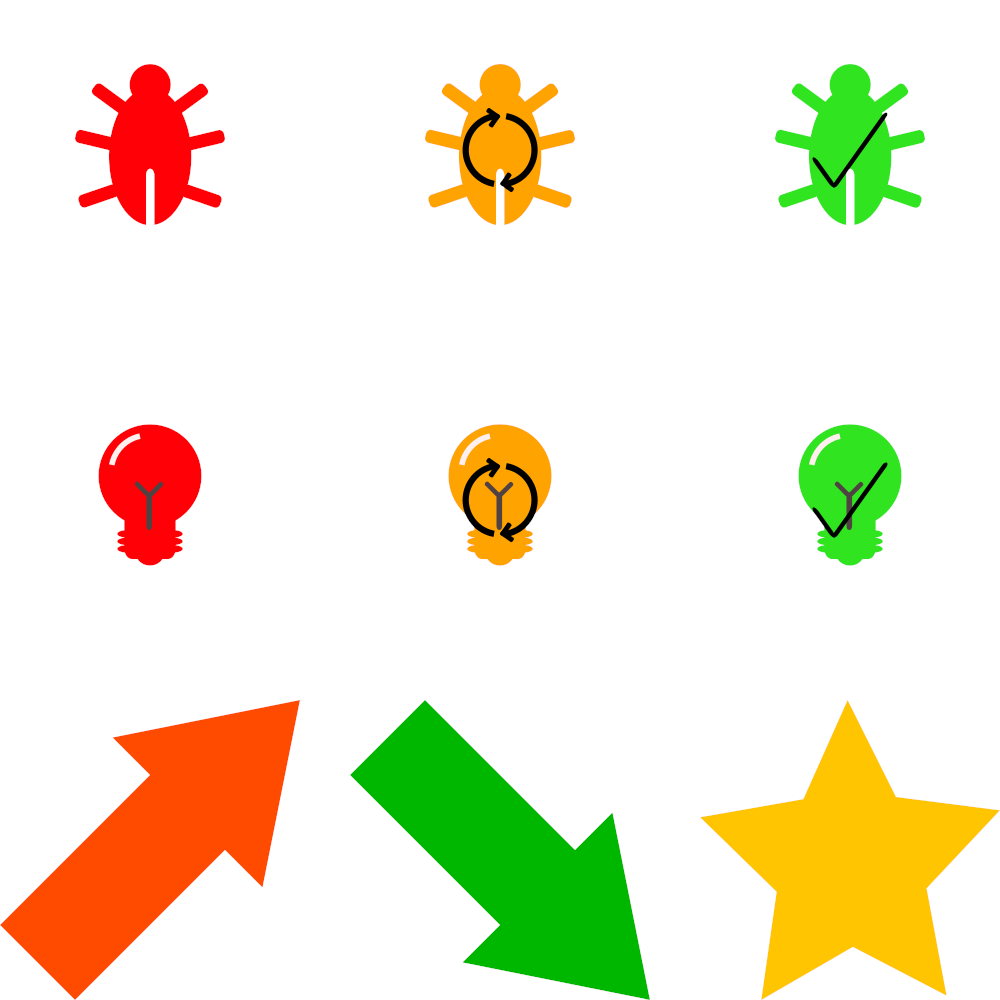
\includegraphics[width=0.5\textwidth]{graphics/iconParts.png}
	\caption{Issue Icon Parts}
	\label{fig:c4:icon_parts}
\end{figure}
\Cref{fig:c4:icon_parts} shows all the parts described above.
The first row contains the bugs in all three possible states, open, work-in-progress, and closed.
In the second row are the enhancements with the same three states.
The third row contains the annotations for the other three properties.
The first annotation is used when this issue is the cause of another issue in some other component.
In the finished icon, it is located in the top right corner.
The second symbol is the annotation for when the issue is caused by another issue and is, therefore, just a symptom of that issue.
On the final icons, this is shown in the top left.
The third symbol represents the fact that the issue is assigned to the current developer.
It is added in the bottom left of the final icon.

\begin{figure}[!h]
	\centering
	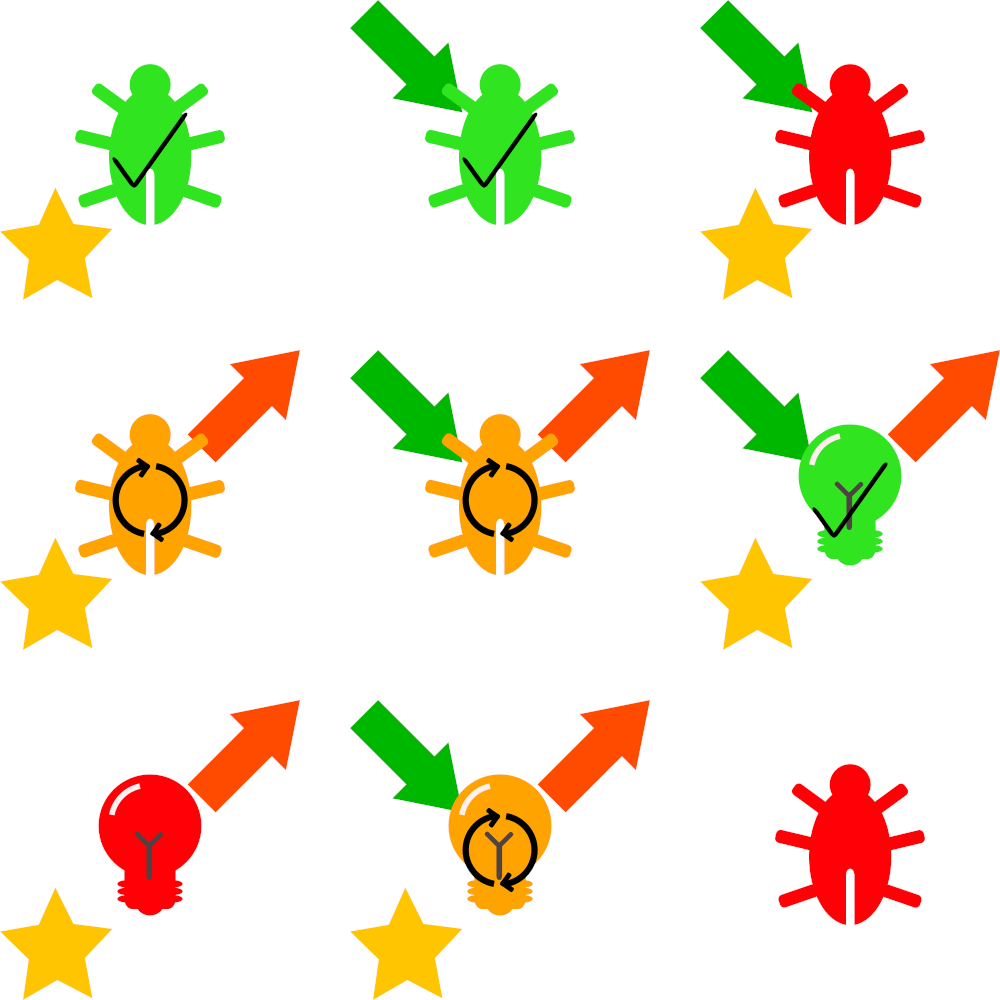
\includegraphics[width=0.5\textwidth]{graphics/iconCombinations.png}
	\caption{Issue Icon Examples}
	\label{fig:c4:icon_combinations}
\end{figure}
In \cref{fig:c4:icon_combinations} some examples of the final icons can be seen.
In total, there are 48 different combinations of the above parts.
All of those need to be created and then converted into a pixel-based image format in multiple sizes so they can be used.
This would be a very tedious manual task for one person.
Especially, as the icons were changed multiple times during the development process.
Therefore, a small script was created, which does all that automatically and results in a folder with all combinations as \gls{PNG} files in the specified sizes.

\section{Eclipse Plugin Architecture}
\label{sec:ch4:s3}
One possible approach that was investigated is to implement the plugin as an extension to Mylyn.
As described in \cref{ssec:ch2:ss2.3}, Mylyn is an \gls{Eclipse} plugin for managing tasks and can, therefore, also be used to manage plugins.
However, many of the required features from \cref{sec:ch3:s1} could, to our knowledge, not be implemented in a Mylyn extension without contributing some significant changes to Mylyn itself.
Any changes proposed for Mylyn would need to be discussed with the community and justified to the maintainers causing, in the best case, a major delay for the implementation of the extension.
In the worst case, some changes may be rejected entirely, preventing the implementation of some of the required features.
Therefore, it was decided to create a new \gls{Eclipse} extension.

As described in \cref{sec:ch3:s3}, the plugin is split into several components for portability reasons.
Therefore, the prototype actually consists of a total of four eclipse plugins, as can be seen in \cref{fig:c4:component_diagram}.
Moreover, it was decided to use a model-driven software development approach similar to the one described by Beydeda et al. \cite{beydeda2005model}.
As a big part of the tool is a list and form for viewing and manipulating data, which can be described formally,
large parts of these two \gls{UI} elements can be automatically generated that way.

\begin{figure}[!h]
	\centering
	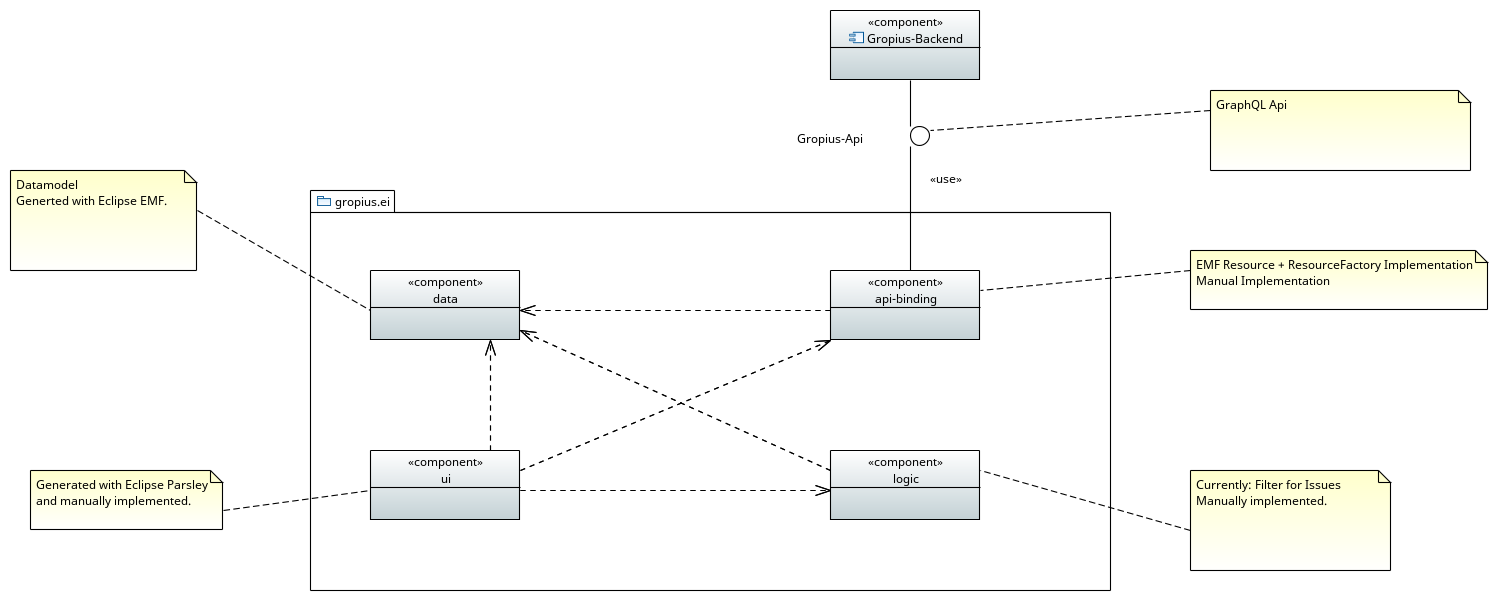
\includegraphics[width=\textwidth]{graphics/Component_Diagram.png}
	\caption{Component Diagram of the Eclipse Extension}
	\caption*{\footnotesize{The same figure can be found enlarged in \cref{chap:appendix:design_docs}}}
	\label{fig:c4:component_diagram}
\end{figure}

The plugin on the top left of \cref{fig:c4:component_diagram}, called \lstinline|data| contains the data model for the plugin. 
It is first modeled as an \gls{UML} model, then converted to an \gls{EMF} ecore model, and then the model code is generated based on that.
Ecore is the metamodel to represent models in the \gls{EMF} world \cite{steinberg2008emf}.

The plugin \lstinline|api-binding| is responsible for all communication with the \gls{Gropius} back-end through the \gls{Gropius} \gls{API}.
Additionally, it converts between the data format defined in the \lstinline|data| plugin and the format used by the \gls{API}.
As mentioned in \cref{ssec:ch2:ss1.2}, the \gls{API} provided by the Gropius system uses \gls{graphql}.
Therefore, the client needs to specify exactly what data is required and create mutations for any changes to be sent to the server.
To be able to create these mutations, the difference between the old and the new version of the change needs to be recorded.
Both the specification of the required data and the creation of mutations is also done by this component.

The third plugin, just called \lstinline|ui|, implements all the \gls{UI} elements.
It is the only plugin of the four that directly interacts with the \gls{Eclipse} \gls{IDE}.
This way, it is the only plugin, which needs major changes when the tool is ported to another \gls{IDE}, which supports Java-based plugins.
It uses the \gls{Parsley} framework introduced by Lorenzo Bettini \cite{bettini2014developing} to generate the issue list and issue details view 
based on the data model from the \lstinline|data| component.

The \lstinline|logic| plugin holds all classes containing logic needed by the \lstinline|ui|, which is not \gls{Eclipse} specific.
One example would be the classes for filtering the issues based on some properties.
They are used by the filters for the issue list but do not require any \gls{IDE} specific functions.

A separate \gls{Eclipse} plugin for the messaging component would likely make sense.
However, it was not modeled, as the idea of the messaging component was dropped from this thesis for time constraint reasons.

\begin{figure}[!h]
	\centering
	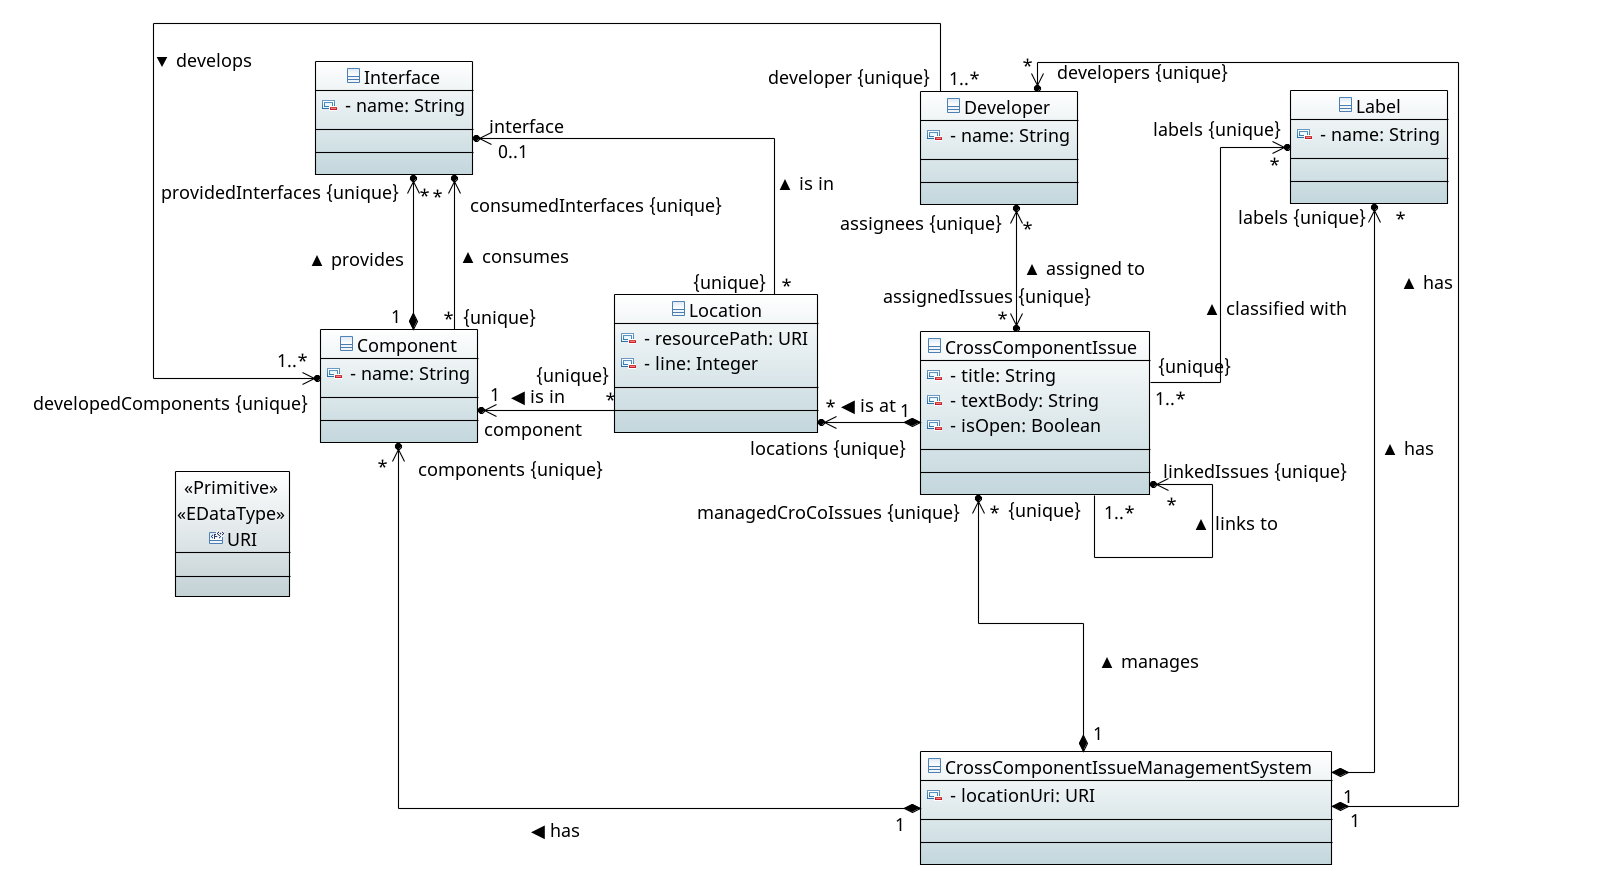
\includegraphics[width=\textwidth]{graphics/dataClassDiagram.png}
	\caption{Class Diagram of the Data Model}
	\caption*{\footnotesize{The same figure can be found enlarged in \cref{chap:appendix:design_docs}}}
	\label{fig:c4:data_class_diagram}
\end{figure}
The class diagram of the data model for \gls{GropiusEI} used to generate the \lstinline|data| component can be seen in \cref{fig:c4:data_class_diagram}.
It is based on the Domain Meta Model shown in \cref{ssec:ch2:ss1.2}.
At the core of the data model is the \lstinline|CrossComponentIssue|, with a title, text body, and a flag indicating whether it is open.
Additionally, it has various references to other objects, such as the assigned developers.

All \lstinline|CrossComponentIssue|s are contained within a \lstinline|CrossComponentIssueManagementSystem|.
That also has a list of all Labels, Developers, and Components relevant for the associated issues.
The tool always works with the issues contained in exactly one \lstinline|CrossComponentIssueManagementSystem|.

One important reference for the functionality of the tool is the \lstinline|linkedIssues| list of a \lstinline|CrossComponentIssue|.
It allows \gls{GropiusEI} to show users linked issues as well as letting users navigate between them.

Another core concept of this model are the \lstinline|Location|s.
One issue can be at zero or more \lstinline|Location|s, which specify the resource and line the \lstinline|Location| is at.
Additionally, a \lstinline|Location| can be in a \lstinline|Component| or an \lstinline|Interface|.
\lstinline|Interface|s can be provided by exactly one \lstinline|Component| and consumed by any number of them.

\section{Eclipse Plugin Implementation}
\label{sec:ch4:s4}

During the implementation phase, one of the biggest challenges was to understand and to correctly use \gls{Parsley} as well as \gls{EMF}.
Not a lot of documentation and tutorials could be found for either of them.
However, as both are open source, answers for specific questions could be searched and found in the code itself.
Yet, this process is rather tedious and slow, so a lot of time was spent just looking through these frameworks' source code.

\Gls{Parsley} is well suited for generating default \glspl{UI} for data models.
It has basic support to customize them, 
but very little existing customization already available.
Therefore, a lot of the implementation work during this thesis was improving classes, which already exist in parsley 
and adding new variants of them, which allow further customization.
Most of them could be contributed to \gls{Parsley} after a little cleanup.

\begin{figure}[!h]
	\centering
	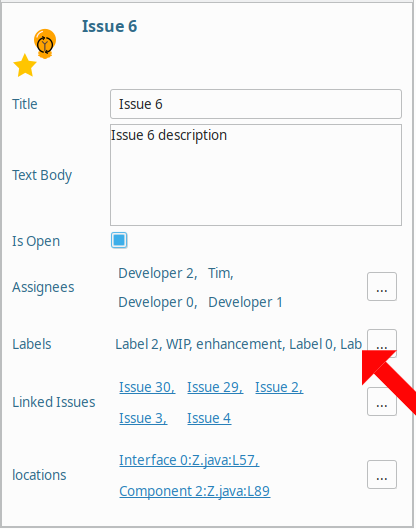
\includegraphics[width=0.5\textwidth]{graphics/screenshot_improvement_fromControl_arrow.png}
	\caption{Difference between original and new Control for Lists}
	\label{fig:c4:screenshot_improvement_formControl}
\end{figure}
One example is the \gls{UI} element displayed inside a form for the value of properties, which are lists.
Parsley only supports to display the string representation of the complete list in one label.
The new implementation of the same class allows child classes to customize this by overwriting some methods.
Based on this, some other classes were implemented using a grid of controls instead of a single label.
This allows for nicer formatting when there are too many elements for one line.
Additionally, this allows the use of links as the control for each element, which is used, for example, by the \lstinline|linkedIssues| property.
The difference between the original and the improved version can be seen in \cref{fig:c4:screenshot_improvement_formControl}.
The control for the list \lstinline|Labels| is created by the original, and you can see the last label is not entirely readable.
The other controls are the new ones, with \lstinline|Developers| using a grid of labels and the other a grid of links.

Another significant amount of time was taken by working on the \lstinline|api-binding| plugin.
As the \gls{Gropius} back-end was not ready in time, the component was implemented to work with a simple mock-up of the back-end.
Because of the fact, that the data from the \gls{API} is transformed into the data model generated with \gls{EMF}, 
the \gls{graphql} \gls{API} cannot be used as intended.
Instead, all relevant data needs to be queried at once every time the data is reloaded from the server.
This problem was detected too late to change the overall architecture of the plugin, 
mainly because the decision to switch to \gls{graphql} for the \gls{Gropius} \gls{API} was made after the concept for \gls{GropiusEI} was already done.
However, to achieve this, a complex query needs to be sent to the server.
Additionally, no appropriate \gls{java} library could be found for using \gls{graphql} \glspl{API} without manually generating the queries and manually parsing the responses. 
In the end, some open-source ruby scripts\footnote{\url{https://github.com/Shopify/graphql_java_gen}} were used to generate helper classes from the \gls{Gropius} \gls{graphql} schema.
The next problem was, that the mock-up of the back-end used to implement the \lstinline|api-binding| component is not sophisticated enough.
The returned data is not consistent in itself, preventing a correct transformation into the \gls{GropiusEI} data model.
As the real back-end would not be ready in time, the decision was made to halt implementing the \lstinline|api-binding| plugin for now.
For the remainder of the thesis, the data is generated by a mock-data generator and stored in a file instead.

\subsection{The Prototype}
Due to the lack of time, many of the features described in \cref{sec:ch3:s3} were not implemented.
Everything that was implemented is presented in the next few paragraphs.

\begin{figure}[!h]
	\centering
	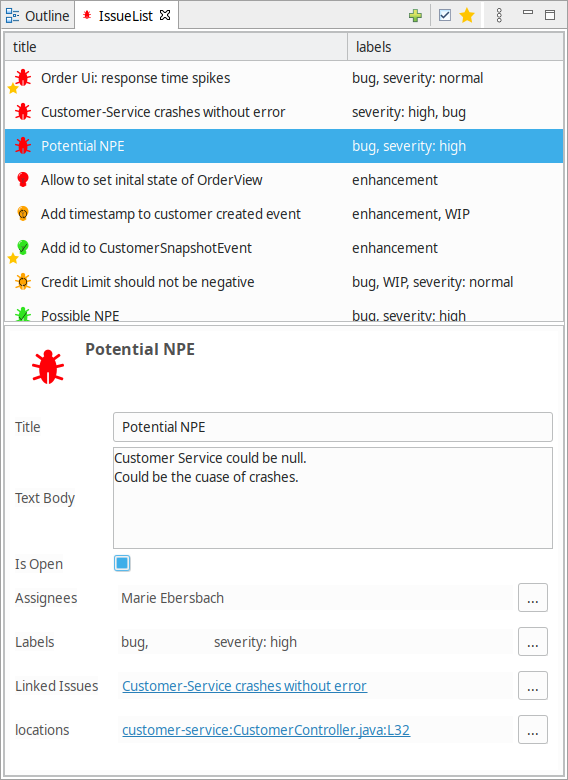
\includegraphics[width=0.45\textwidth]{graphics/screenshot_gropius_ei_issue_list.png}
	\caption{Prototype Issue List}
	\label{fig:c4:screenshot_issue_list}
\end{figure}

As stated in \cref{sec:ch3:s3} the main elements of \gls{GropiusEI} are the issue list and the issue detail view.
Deviating from the concept, those two elements are implemented in one big view element, as shown in \cref{fig:c4:screenshot_issue_list}.
This is the case because \gls{Parsley} provides such a view, and implementing interactions between the two parts is easier that way.
The issue list is in the upper half of the picture. 
It consists of multiple columns, each responsible for one property of the issues.
By default, only the title and label columns are shown, but the user can change this through the menu on the top right.
In theory, all properties that can be seen in the form in the lower half of the image can also be displayed as columns in the list.
However, especially the text body does not make much sense to be displayed in the list, as it can take a lot of space.
In the first column of the list, the icons from \ref{sec:ch4:s2} are displayed in addition to the property of that column.
Currently, the annotations for this issue being caused by another or causing another issue are not used because that feature has not yet been implemented.
The entries of columns with a list of values are not sorted in any way but display the values in the order they are contained in the respective list for this property.
This list is initially ordered by when the value was added but can be reordered by the user in the dialog for editing that property.

As you can see in \cref{fig:c4:screenshot_issue_list_filtered_sorted}, the issue list also supports sorting by a column.
This is done by clicking on the column header.
Furthermore, filtering is supported using the buttons in the bar on the top edge of the view.
Currently, only the filters \lstinline|Only show open issues| and \lstinline|Only show issues assigned to me| are implemented. 
However, all the other filters specified in \cref{sec:ch3:s3} should be fairly straight forward to include.

\begin{figure}[!h]
	\centering
	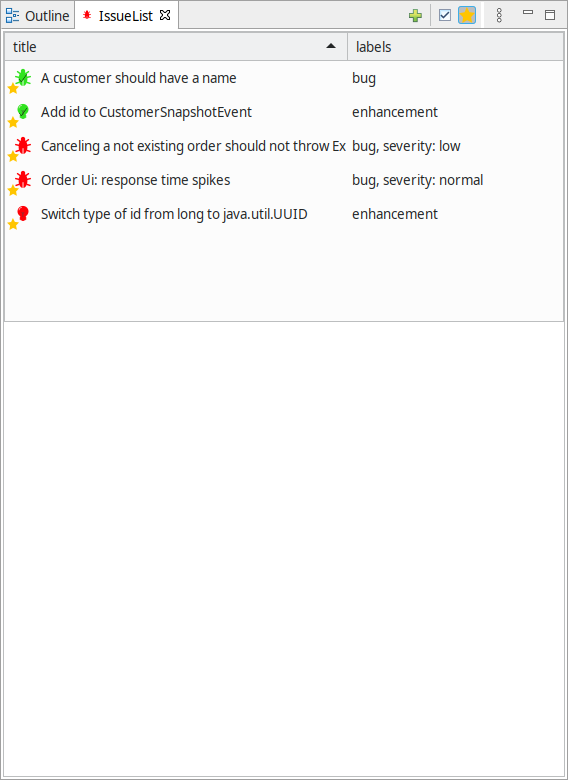
\includegraphics[width=0.45\textwidth]{graphics/screenshot_gropius_ei_issue_list_filtered_sorted.png}
	\caption{Prototype Issue List with Filter and Sorting}
	\label{fig:c4:screenshot_issue_list_filtered_sorted}
\end{figure}

\Cref{fig:c4:screenshot_issue_list} also shows the details view, which additionally is the form for editing a selected issue.
On the top of that form, the icon and the title of the issue can be seen.
Below that, all properties are displayed.
Like the issue list, the properties with multiple values are ordered according to the order in the data instead of being sorted somehow.
For the \lstinline|Linked Issues| and the \lstinline|Locations| each value is a link, 
selecting the correct issue in the list and jumping to that location in the code, respectively.
To change a textual property, the user can simply type in the corresponding text area.
The properties, which contain a list of values, can be modified using the button to the right.

\begin{figure}[!h]
	\centering
	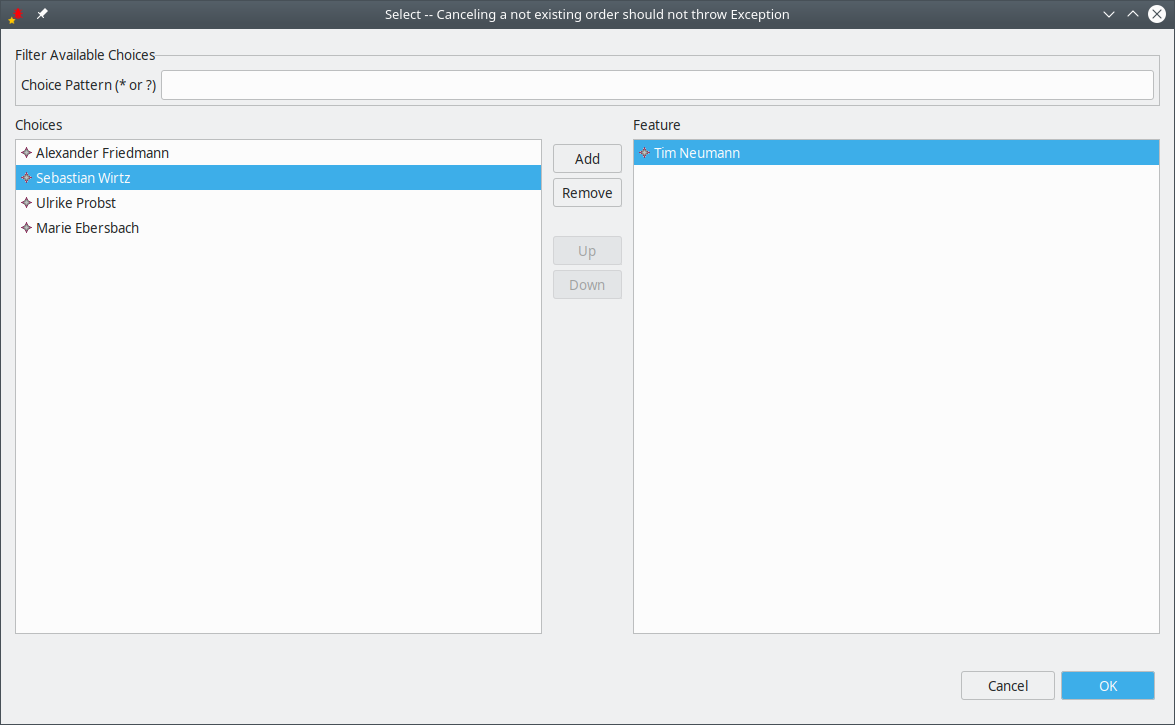
\includegraphics[width=0.8\textwidth]{graphics/screenshot_gropius_ei_edit_list.png}
	\caption{Prototype Edit Developers Dialog}
	\label{fig:c4:screenshot_edit_list}
\end{figure}

When that button is pressed a dialog similar to the one in \cref{fig:c4:screenshot_edit_list} is opened.
With it, the user can select the values for that issue from a list of all possible values for the property.
This dialog also allows the reordering of the values mentioned above.
Changes done in the dialog are applied when the \lstinline|Ok| button is pressed.

\begin{figure}[!h]
	\centering
	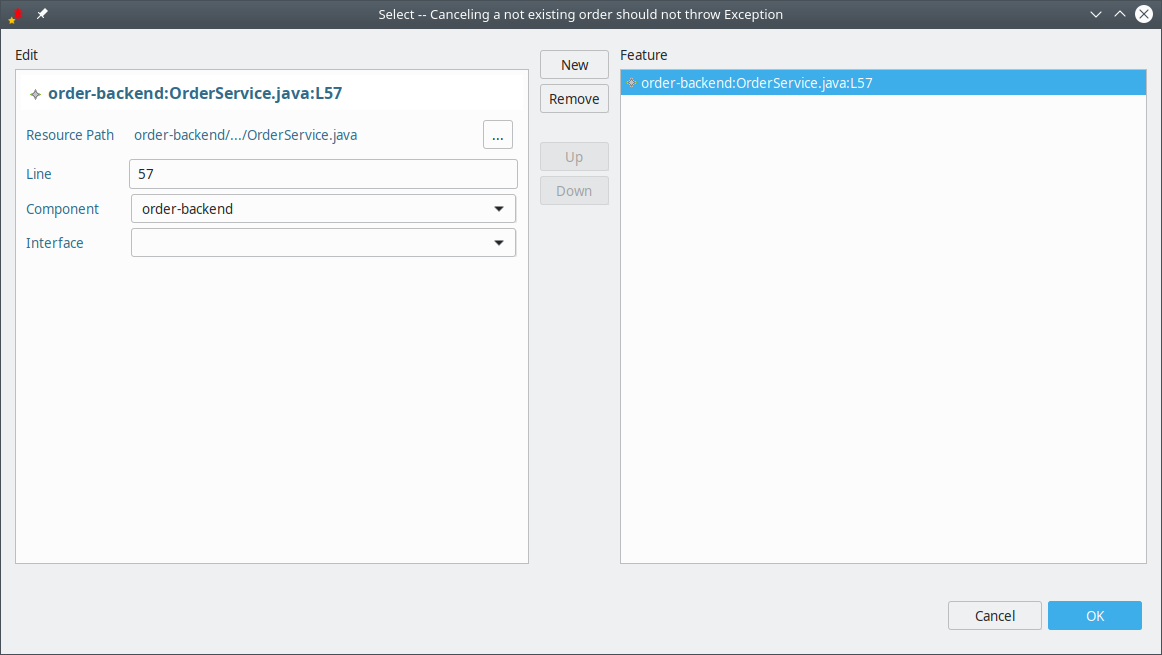
\includegraphics[width=0.8\textwidth]{graphics/screenshot_gropius_ei_edit_locations.png}
	\caption{Prototype Edit Locations Dialog}
	\label{fig:c4:screenshot_edit_locations}
\end{figure}

The only exception for the editing dialogs is the \lstinline|locations| property.
For those a dialog (shown in \cref{fig:c4:screenshot_edit_locations}), which allows creating and editing locations is opened.
Using the \lstinline|New| button, a new location is added to the list of locations for that issue.
Then it, as well as any existing location, can be edited with the left half of the dialog.

After all changes, the issue list is in an unsaved state, indicated by a star in the view name in the tab of the view.
To save the changes, all usual ways to save a resource in \gls{Eclipse} can be used, such as the save button in the toolbar.

The green plus button seen above the issue list in \cref{fig:c4:screenshot_issue_list} can be used to create new issues.
It adds a new issue with empty properties to the list, which can then be edited using the form below.
The feature for creating issues directly from some lines of code has not yet been implemented.

% !TeX spellcheck = en_US

\chapter{Evaluation}
\label{chap:ch5}
For evaluating the usefulness of the prototype an expert review and survey are performed.
To acquire the questions for this survey a process based on the \gls{GQM} approach introduced by \cite{caldiera1994goal} is used.
The results from that are shown in \cref{sec:ch5:s1}.
\Cref{sec:ch5:s2} describes the design and realization as well as the results of the expert review and survey.
In \cref{sec:ch5:s3} the results of the survey as well as the validity of the thesis are discussed.
Finally, the identified threats to this validity are described in \cref{sec:ch5:s4}.

\section{GQM}
\label{sec:ch5:s1}
The process described in this section does not exactly follow the \gls{GQM} approach introduced by \cite{caldiera1994goal},
but is based on it.
The objective of the process is to find good questions, which can be used to evaluate the success of this thesis.
Based on these questions the expert survey can then be performed.

The first step is to identify the goals of the work.
For this thesis, the following could be identified as the primary and only goal \textbf{(G1)}:
Improve the efficiency, effectiveness, and convenience for developers when working with issues in the Gropius environment during their software development process. 

Next, questions have to be found, which can be used to evaluate, whether that goal is reached.
For that purpose the following three questions could be identified:
\begin{itemize}
	\item[\textbf{Q1}] What problems do developers face when working with issues affecting multiple independent projects during the software development/engineering process?
	\item[\textbf{Q2}] Which of these problems does this thesis's tool solve and to which degree?
	\item[\textbf{Q3}] Can the industry imagine using such a tool in production?
\end{itemize}

As it was clear from the start, that an expert review and survey would be conducted, no metrics need to be found for these questions.
However, it must be investigated if an expert review is a reasonable metric for these questions.
For \textbf{Q1} an expert survey is a reasonable metric if the experts are developers, who currently work are have worked in a field with multiple independent projects or have enough experience to put themselves into that situation.
It is an adequate metric for \textbf{Q2} if the experts fulfill the conditions above and have used the thesis' tool or at least were given an introduction about the features of the tool.
An expert survey is a reasonable metric for \textbf{Q3} if the experts are or have been working in the industry and fulfill the above conditions.

Therefore, the evaluation metric (\textbf{M1}) for all questions is an expert review and survey with the correct experts, who are introduced to \gls{GropiusEI}. 

\section{Expert Survey}
\label{sec:ch5:s2}
The main element of this evaluation is the expert survey, where selected experts answer a set of prepared questions. 
But first, an expert review of \gls{GropiusEI} is performed.
This makes sure the experts know the tool and its features and has the additional benefit of direct feedback about the prototype.
The process of the review and survey is explained in \cref{ssec:ch5:ss2.1}.
The results from both are presented in \cref{ssec:ch5:ss2.2}.

\subsection{Design and Realization}
\label{ssec:ch5:ss2.1}
To perform an expert review and survey, first, a group of experts has to be found.
To achieve this, various developers from academia and industry were contacted and asked to participate in this review.
If they were generally interested, the thesis' concept and the procedure of the review and survey were explained to them.
In total 21 experts were contacted, of which 12 agreed to take part.

As preparation for the expert review, a detailed guide on installing \gls{GropiusEI} was produced
to ensure experts could install it on their own device if they wanted.
It can be found in \cref{sec:appendix:er:install_guide} and
the exact release used for the review is attached as \cref{sec:appendix:er:release}.

Additionally, a scenario was created, in which experts could test the tool in as real as possible conditions.
This scenario consists of an \gls{Eclipse} workspace with a java-based demo software using multiple components \footnote{\url{https://github.com/eventuate-tram/eventuate-tram-examples-customers-and-orders}} and a \gls{GropiusEI} data file.
This data file contains the correct components and interfaces for the workspace as well as some developers and labels in addition to
several invented issues.
These issues are as realistic as possible with a title that could be found in a live \gls{IMS} somewhere, a feasible text body,
typical labels, sometimes linked issues, and most with at least one location in the workspace.
Furthermore, a few tasks were prepared, which were used to introduce each feature to the expert.
These tasks were typical things a developer would need to do during his workday like finding an issue in the code or creating a new issue.
For each task, a detailed explanation, how the task can be done using \gls{GropiusEI} is also included. 
The scenario can be found in \cref{sec:appendix:er:scenario} and a short explanation as well as the mentioned tasks in \cref{sec:appendix:er:scenario_explanation}.

After an expert agreed to participate they were provided with three options for executing the expert review and asked which they preferred.
The first option was to install the tool and the scenario on their device with the help of the mentioned installation guide.
Then an online meeting would be scheduled, such that the tasks from the scenario could be completed while I watch with the help of a screen sharing solution. That way I could help the experts with any problems and directly answer questions as well as guide them through the prepared tasks instead of sending the tasks.
The second option was, that the expert installs both on their device and goes through the scenario doing the tasks on their own.
In this case, they were sent the tasks including the explanations in a written document.
The last option was, that I would present the tool in an online meeting using screen sharing tools. That way the expert did not need to install anything on their device. For that reason, this was also the fastest option. On the other hand, the expert could not use the tool himself, but just watch me do the tasks.
In every case, the expert was asked for general feedback.

After an expert completed the review he was sent the following questions and asked to answer them:
\begin{enumerate}
	\item What do you see as the most significant problems when working with issues affecting multiple independent projects during your software development/engineering process? \label{itm:ch5:expert_questions_problems}
	\item Do you think the following points represent problems or challenges of existing issue management systems you face as a developer? \label{itm:ch5:expert_questions_are_these_problems}
	\subitem The lack of insufficient support of linking issues to multiple specific software development artifacts accurate to the line, especially if the artifacts are part of multiple independent projects.
	\subitem The lack of insufficient support of linking issues to each other
	\subitem The lack of inadequate support of navigating from one to the next issue through the chain of related or dependent issues.
	\item For which of these problems (from points 1 and 2) would you say Gropius EI completely solves them? \label{itm:ch5:expert_questions_solve}
	\item For which of these problems (from points 1 and 2) would you say Gropius EI reduces them? \label{itm:ch5:expert_questions_reduce}
	\subitem How far would you say are each of these problems reduced?
	\item Could you imagine to use Gropius EI in your day-to-day business?
\end{enumerate}
These questions are based on the evaluation questions \textbf{Q1} to \textbf{Q3} presented in \cref{sec:ch5:s1}.
Question \ref{itm:ch5:expert_questions_are_these_problems} was added in order to get good answers to questions \ref{itm:ch5:expert_questions_solve} and \ref{itm:ch5:expert_questions_reduce} even if the expert did not find a lot of answers to question \ref{itm:ch5:expert_questions_problems}.
The points for question \ref{itm:ch5:expert_questions_are_these_problems} were conceived in an internal brainstorming session.

\subsection{Results}
\label{ssec:ch5:ss2.2}
%Of the 12 experts, who agreed to participate, a total of $x$ reviewed the tool and $y$ answered the prepared questions in the end. \todo{Insert correct numbers}
\section{Discussion}
\label{sec:ch5:s3}
\section{Threats to Validity}
\label{sec:ch5:s4}

\begin{figure}[!h]
	\centering
	\tikzset{
		my node style/.style={
			font=\small,
			rectangle,
			rounded corners,
			minimum size=6mm,
			drop shadow,
			draw=blue!40, 
			fill=blue!20, 
			very thick,
			align=center,
		}
	}
	\forestset{
		my tree style/.style={
			for tree={
				my node style,
				parent anchor=south,
				child anchor=north,
				l sep+=5pt,
				edge={draw=blue!40, very thick},
				edge path={
					\noexpand\path [draw, \forestoption{edge}] (!u.parent anchor) -- +(0,-7.5pt) -| (.child anchor)\forestoption{edge label};
				},
			    delay={if content={}{shape=coordinate}{}}
			}
		}
	}
	\begin{forest}
	my tree style
	[Threats to Validity
      [External Validity
	    [\begin{varwidth}{0.16\linewidth}Small sample size\end{varwidth}]
	    [\begin{varwidth}{0.16\linewidth}Sample not representative\end{varwidth}]
	  ]
	  [Construct Validity 
	    [[[
	      [\begin{varwidth}{0.16\linewidth}Questions for experts misrepresent research questions\end{varwidth}]
	      [\begin{varwidth}{0.16\linewidth}Questions misunderstood by experts\end{varwidth}]
	      [\begin{varwidth}{0.16\linewidth}Answers misinterpreted\end{varwidth}]
	      [\begin{varwidth}{0.16\linewidth}Only one kind of measurement\end{varwidth}]
	      [\begin{varwidth}{0.16\linewidth}Expert survey is not objective nor statistical\end{varwidth}]
	    ]]]
	  ]
	  [Reliability
	      [\begin{varwidth}{0.16\linewidth}Documents written in German\end{varwidth}]
	      [\begin{varwidth}{0.16\linewidth}Artifacts hosted online may not be available forever\end{varwidth}]
	  ]
	  %[Internal Validity]
	]
	\end{forest}
  
	\caption{Overview over the Threats to Validity}
	\label{fig:threatsToValididty}
\end{figure}

This section discusses which threats to the validity of the results discussed above could be identified.
An overview of these threats can be seen in ...
The threats can be grouped into four categories as stated by \cite{runeson2009guidelines}.

The first category investigated, is internal validity.
This aspect of validity is concerned with whether the observed results are actually caused by the changes introduced by this work,
or if the results could be the effects of any unknown influence \cite{runeson2009guidelines}.
But as the experts were directly asked if \gls{GropiusEI} solves or reduces the stated problems, no threat to this aspect of validity could be identified.

The next kind is construct validity.
It represents the correctness of the assumption, that the collected results actually correspond to the research questions \cite{runeson2009guidelines}.
For this aspect, a few threats could be identified.
First, the questions sent to the experts, which are presented in \cref{ssec:ch5:ss2.1} could misrepresent the research questions 
introduced in \cref{sec:ch5:s1}.
Next, these questions could have been misunderstood by one or more experts.
Furthermore, the answers of the experts could have been misinterpreted.
Moreover, just a single kind of measurement was performed.
Finally, an expert survey does not produce objective ore statistical results.
The results are subjective answers from the experts given in free text form, such that statistical evaluation is difficult. 

Another aspect is the external validity.
That is concerned with whether the results can be generalized beyond the small studied sample \cite{runeson2009guidelines}.
The following threats were identified for this category:
First, the sample size was very small compared to all developers working with issues in a relevant field.
Second, the experts were not picked randomly, but all had prior contact with me or my supervisor.
Therefore, the sample was not very representative of the complete population.

The last aspect of validity is reproducibility or reliability.
It deals with any reasons a separate evaluation by other researchers reproducing this evaluation would not have the same conditions \cite{runeson2009guidelines}.
For this aspect, no major threats could be identified, as the whole process is described in detail in \cref{ssec:ch5:ss2.1} and all artifacts used can be found in \cref{chap:appendix:expert_review_docs}.
The first minor threat found, is the fact that these documents are written in German and would need to be translated for researchers or experts who don't speak German.
The other minor threat is that the artifacts hosted on the internet referenced in the appendix might not be available forever.
% !TeX spellcheck = en_US

\chapter{Conclusion}
\label{chap:ch6}
This chapter concludes this thesis, by first giving a short summary in \cref{sec:ch6:s1}, highlighting the most important lessons learned during the process of this thesis in \cref{sec:ch6:s4}, and finally discussing what work could be based on this thesis in the future in \cref{sec:ch6:s5}.

\section{Summary}
\label{sec:ch6:s1}
The goal of this thesis was to develop, implement, and evaluate a concept for integrating \gls{Gropius} into the developer's \gls{IDE} and therefore improve the efficiency, effectiveness, and convenience for developers when working with issues in environments with many components and multiple teams during their software development process.

First, a concept for such an \gls{IDE} extension was developed based on a requirements engineering process.
This concept is independent of the \gls{IDE} and can therefore be used to develop an extension for any \gls{IDE}.
At the core of the concept is the issue list and the issue detail \gls{UI} element.

Then, an \gls{Eclipse} extension has been implemented based on this concept.
Large parts of it are created using a \gls{MDSD} approach, therefore a lot of the code is generated.
Even though various features could not be implemented in time, the result helps demonstrate the concept.
It can easily be developed into a full issue management extension using \gls{Gropius}.

Using this extension an expert review has been performed followed by an expert survey.
The former was used to gain feedback about the extension while the latter served as the evaluation of the concept.
While the experts generally like the concept not all see the problems it is trying to solve.
However, most experts do agree with at least some of the problems and think \gls{GropiusEI} does solve them.
Finally, all but one expert can imagine using it in the future.
Based on the discussion of these results it can be said, that the thesis' goal is reached.

In the end, this thesis provides a detailed concept for issue management plugins working with the \gls{Gropius} framework as well as a basic implementation of it together with a lot of feedback for future improvements.

\section{Lessons Learned}
\label{sec:ch6:s4}
The most important thing I learned during the process of this thesis is using a \gls{MDSD} approach 
and especially working with \gls{EMF} and especially \gls{Parsley}.
Both do not have a lot of documentation, but by working with them and looking into their source I learned a lot about their use but also their internals.

Additionally, I gained practical experience with planning and performing an expert review and survey.
Especially creating the research questions using the \gls{GQM} approach and evaluating the threats to validity gave me a lot of insight into those areas.

Moreover, I also practiced and improved my literature research as well as scientific writing skills.
I especially learned searching in an area with very little scientific work and finding hidden papers.

\section{Future Work}
\label{sec:ch6:s5}
One possible first step for any future work is obviously improving \gls{GropiusEI}.
The remaining features proposed in the concept, as well as the ones suggested by the experts, could be implemented.
Once the extension is in a more usable form and the \gls{Gropius} back-end also has support for some \gls{IMS},
a study with many more developers could be performed in one or more companies.
An instance of the back-end could be set up within each company and linked to their existing \glspl{IMS} and other \gls{IMS} of projects they are using.
Then, the developers of the company could try using \gls{GropiusEI} in their daily business.
This study could reveal the performance increase gained by using the extension.

Alternatively, extensions for other \glspl{IDE} could be developed based on the concept of this thesis.
This helps to evaluate how easily it can be applied to those other \glspl{IDE} and how much work needs to be done to port the existing \gls{IDE}-independent parts of the extension to another extension.
It would need to be evaluated if it is easier to get the code generated by \gls{EMF} working with another \gls{IDE} or if it is easier to generate new code from the existing models with the help of another \gls{MDSD} framework. 

\printbibliography

All links were last followed on August 17, 2020.

\appendix
%\input{latexhints-english}

\pagestyle{empty}
\renewcommand*{\chapterpagestyle}{empty}
\Versicherung
\end{document}
